\chapter{Naughty maid}
Naughty maid is the adult theme app name of the remaining four malware samples analyzed. The objective of the virus is to log to a remote chinese server sensitive information like position and stored files and, in addition, can make the phone subscribe to paid SMS services  and cancel the SMS afterwards to hide its malicious behavior.

\section{File differences}
As previously stated we received four jar files identified by their SHA256 hash:
\begin{itemize}
	\item \texttt{0b8bae30da84fb181a9ac2b1dbf77eddc5728fab8dc5db44c11069fef1821ae6}
	\item \texttt{0b41181a6b9c85b8fa5c8e8c836ac24dd6e738a0d843f0b81b46ffe41b925818}
	\item \texttt{0c05e5035951e260725d15392c8792a4941f92f868558e8b90b52977d832a70d}
	\item \texttt{0c40fb505fb96ca9aed220f48a3c6c22318d889efa62bc7aaeee98f3a740afab}
\end{itemize}
 
To make sure they were part of the same family of viruses, we used a jar compare tool confirming that most of the source files were practically identical. Only \texttt{0c05..} presented slightly more differences, mainly in the \texttt{AndroidManifest.xml} file, but otherwise remained the same w.r.t. the other files (Fig. \ref{fig:jarCompare}).

\begin{figure}[h!]
\centering
    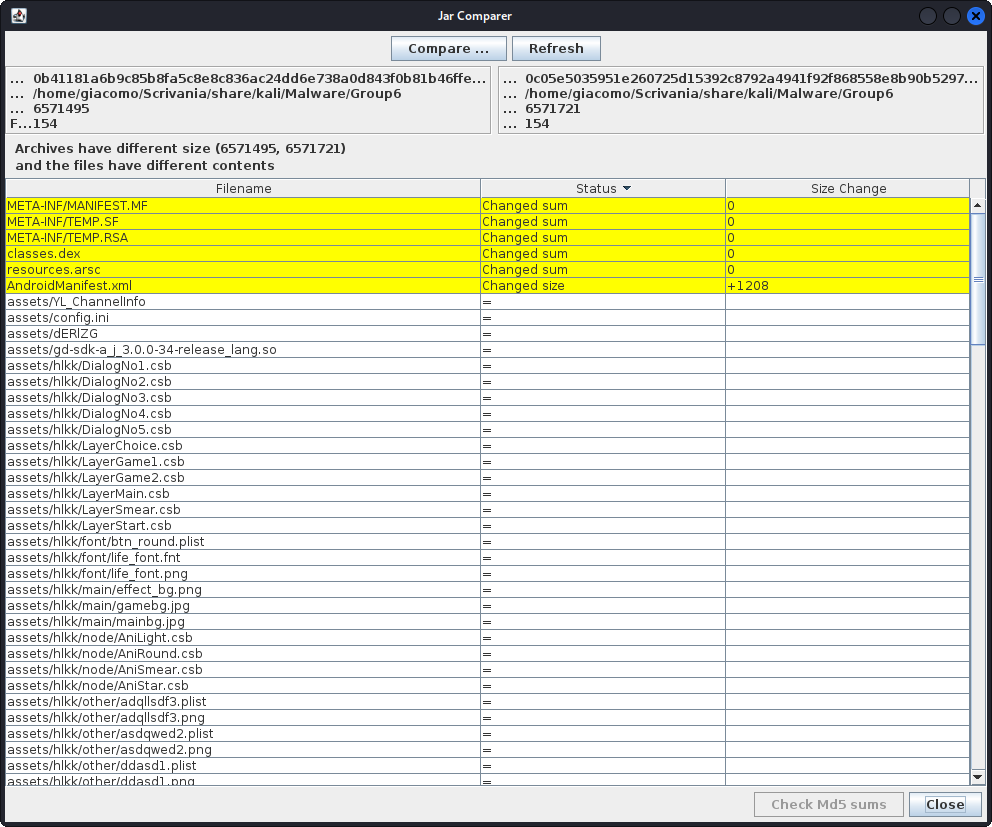
\includegraphics[width=1\textwidth]{./images/screenshot/jarcompare/jarCompare.png}
    \caption{jarCompare output}
    \label{fig:jarCompare}
\end{figure}

From this point forward we will always reference the \texttt{0c05..} sample file and its content when speaking about this virus family and, if there will be any differences with the other samples, they will be pointed out.

\section{Static Analysis}

As with SanaSystem, we firstly fed the obtained APK to virus total and got the following result shown in Fig. \ref{fig:MaidReview}.
\begin{figure}[h!]
\centering
    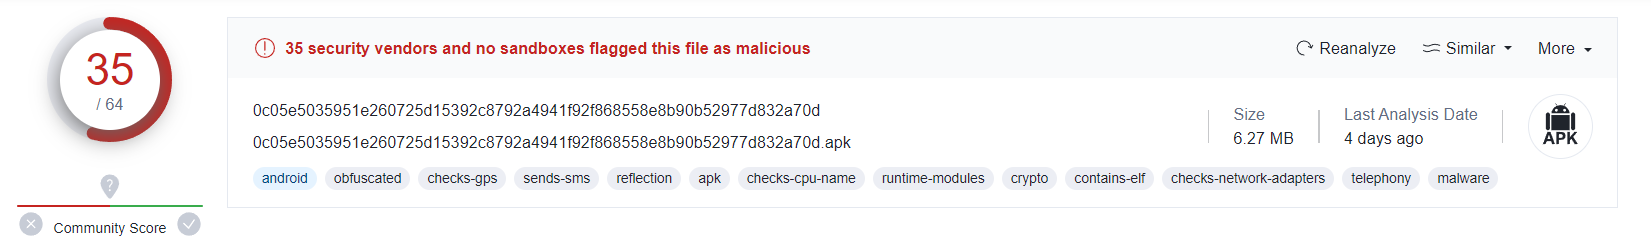
\includegraphics[width=1\textwidth]{./images/screenshot/NaughtyMaid/Review.png}
    \caption{Virus total review}
    \label{fig:MaidReview}
\end{figure}

All samples scored 35/64 execpt for the \texttt{0c40..} file that received a score of 33/59, this indicates that, even if the files are practically the same, even small changes can affect the malware fingerprint which changes its detectability from anti-viruses. In particular a common anti-malware such as MalwareBytes was not able to recognize the software as malicious in every case. As show in Fig. \ref{fig:MaidDetection} the virus is categorized as trojan.smsreg/andr same as the other ones except for 0c40 which is classified as trojan.smsreg/smspay. The first one identifies an app disguised as a legit one with the malicious goal of collecting user and phone data, the second one identifies an app whose goal is to subscribe the phone to premium sms services and hide its functionality by deleting the incoming malicious sms. As previously stated the 4 files are basically the same malware and this difference in categorization implies a high range in malicious activity, this is also implied by the permission required shown in Fig. \ref{fig:MaidPermission}.

\begin{figure}[h!]
\centering
    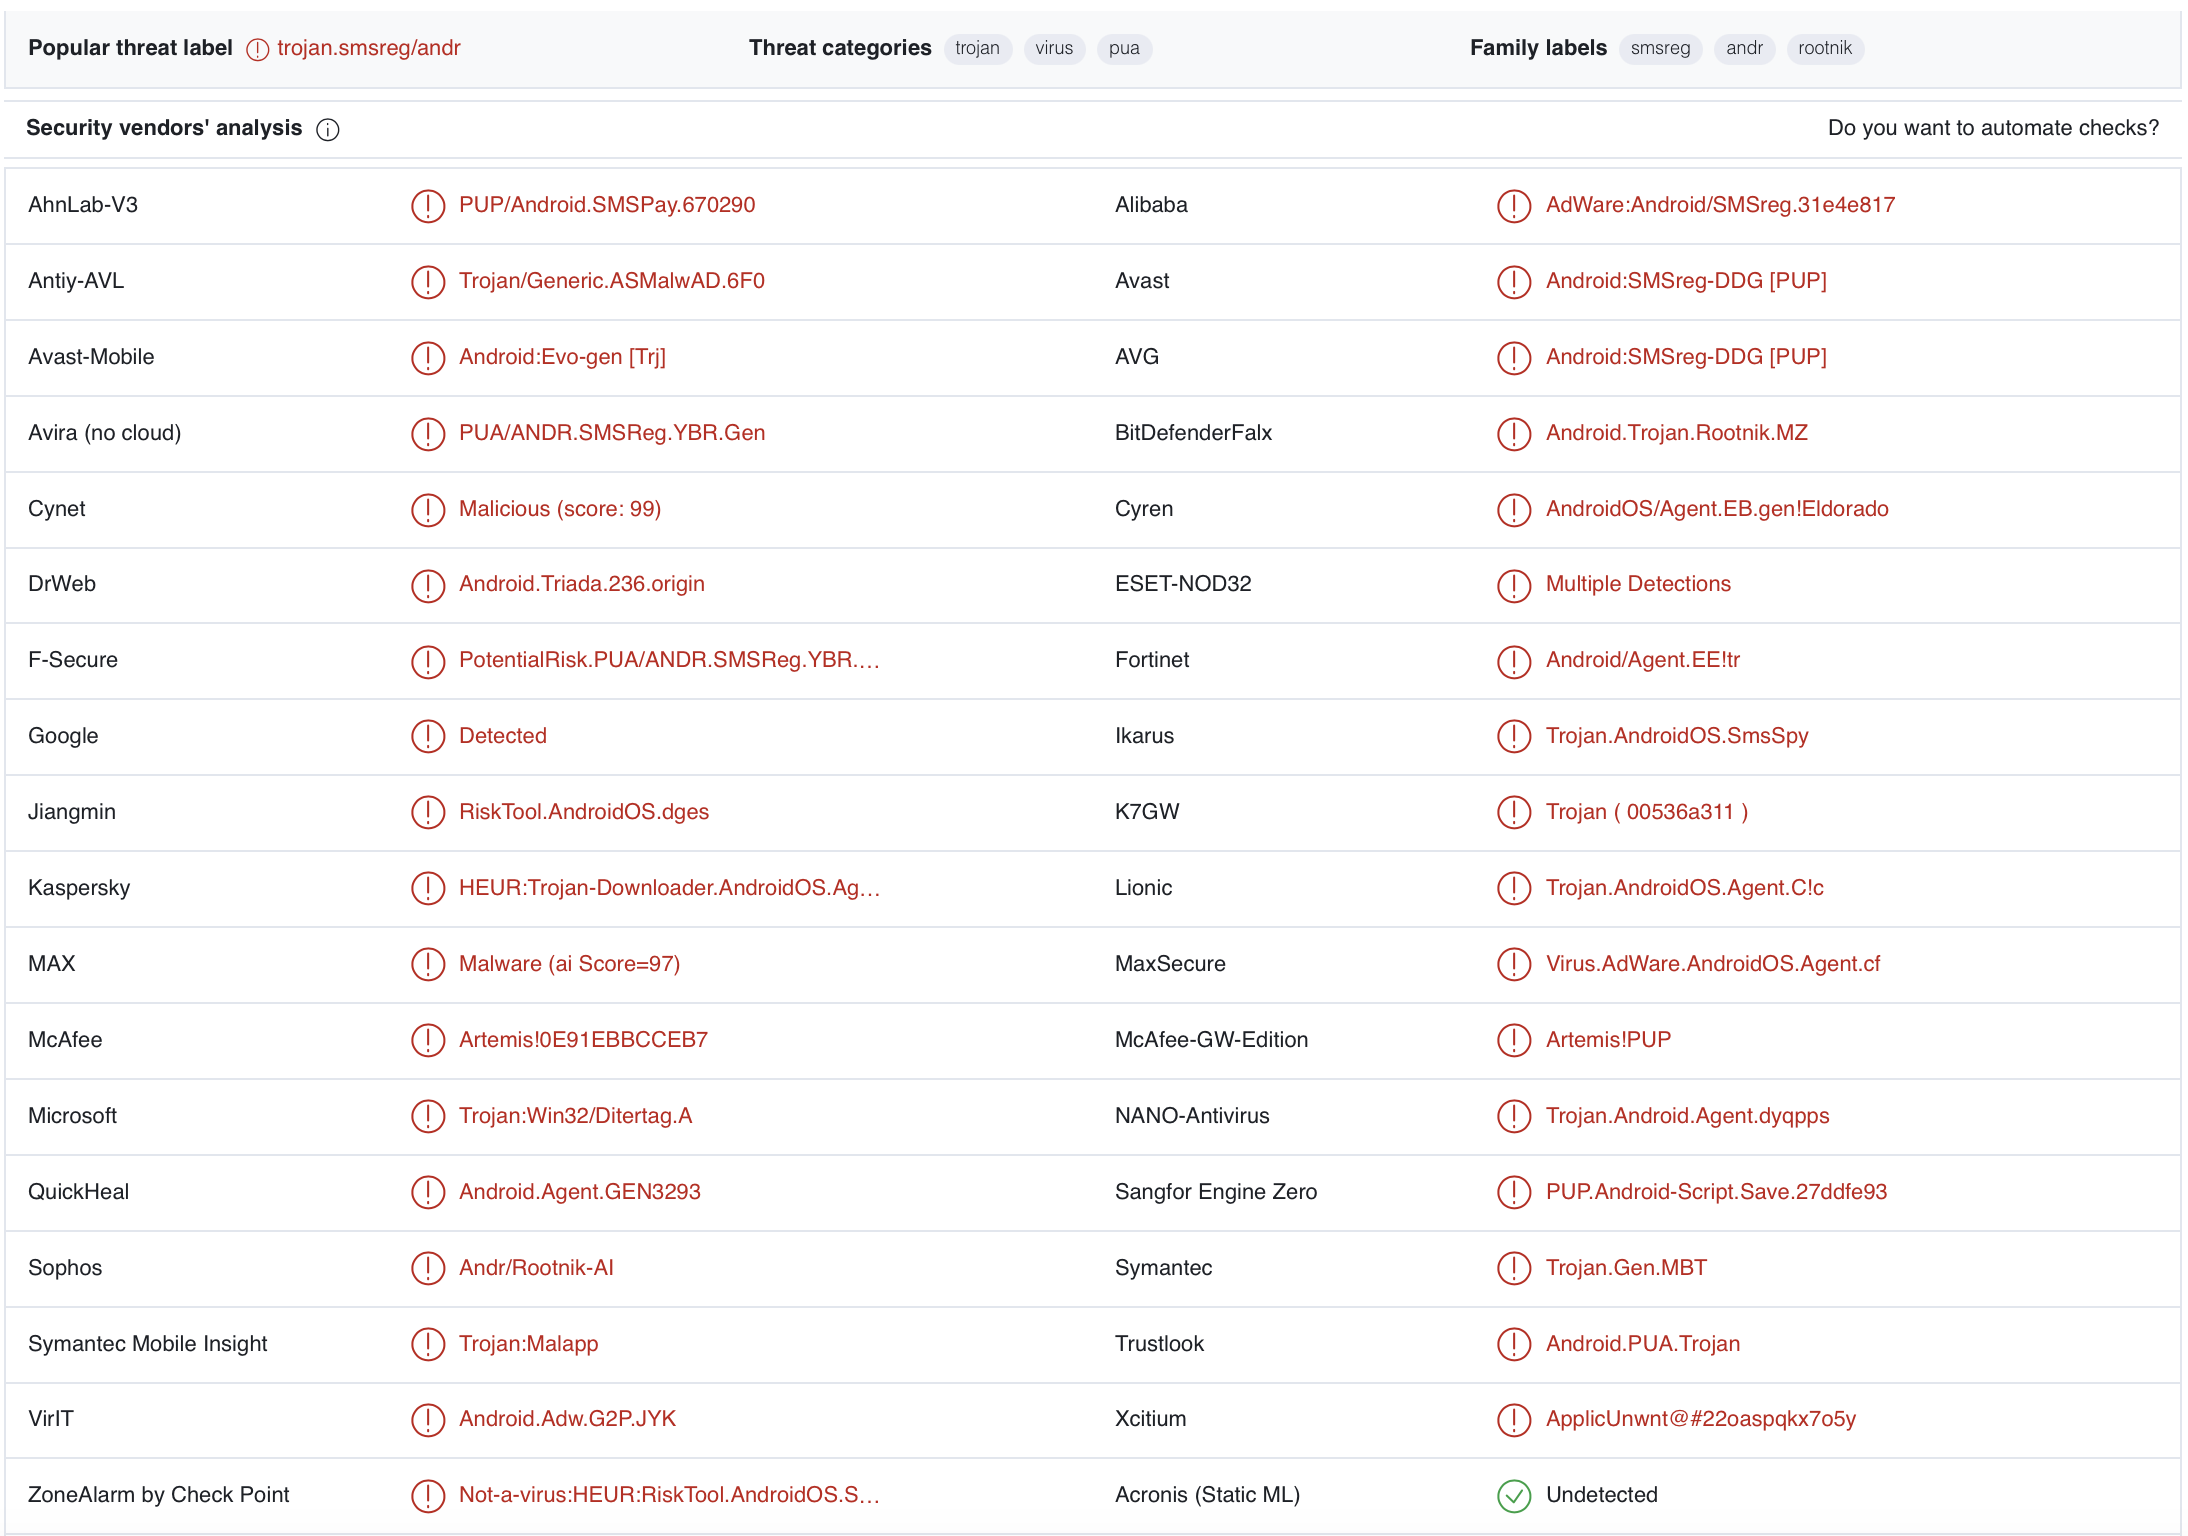
\includegraphics[width=1\textwidth]{./images/screenshot/NaughtyMaid/Detection.png}
    \caption{Virus total detection}
    \label{fig:MaidDetection}
\end{figure}

\begin{figure}[h!]
\centering
    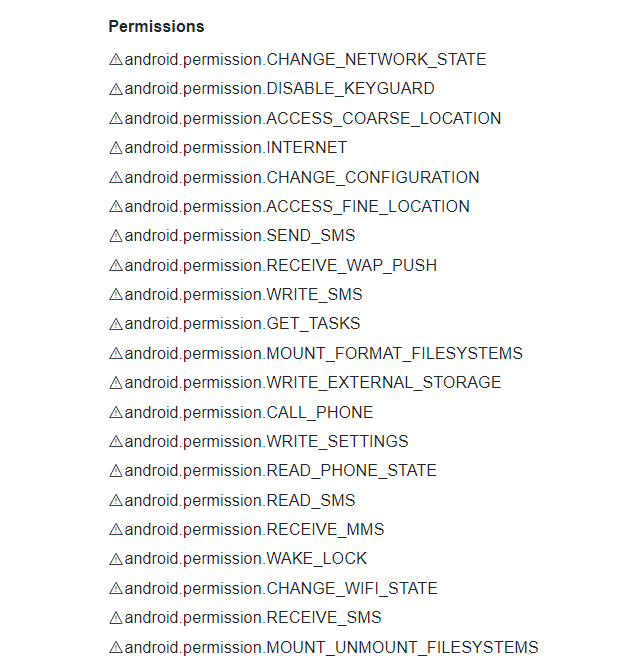
\includegraphics[width=0.5\textwidth]{./images/screenshot/NaughtyMaid/Permission.png}
    \caption{NaughtyMaid permission}
    \label{fig:MaidPermission}
\end{figure}

\subsection{URL and domains}
MobSF also indicated the presence of many hardcoded URL and relative domains Fig. \ref{fig:MaidDom1} \ref{fig:MaidDom2} \ref{fig:MaidDom3} \ref{fig:MaidDom4} \ref{fig:MaidDom5}. Many of them are located in China and, after a quick check with a DNS lookup and an IP lookup tools, it was revealed that other domains not identified by MobSF are located there. Others were misidentified and placed in European countries such as \emph{alog.umeng.com} that was signaled to be hosted in Frankfurt when in reality it resides in Honk Kong at the time of writing this report. 

Regarding the URLs, there are too many to be presented in a single list so we decided to report the most suspicious ones, please note that these may be more malicious URLs, however these four are those with the most suspicious names.
\begin{itemize}
	\item http://118.85.194.4:8083/iapSms/ws/v3.0.1/mix/billing
	\item http://139.129.132.111:8001/CrackCaptcha/GetCaptchaValue.aspx
	\item http://pay.918ja.com
	\item http://vpay.api.eerichina.com/api/payment
\end{itemize}

\begin{figure}[h!]
\centering
    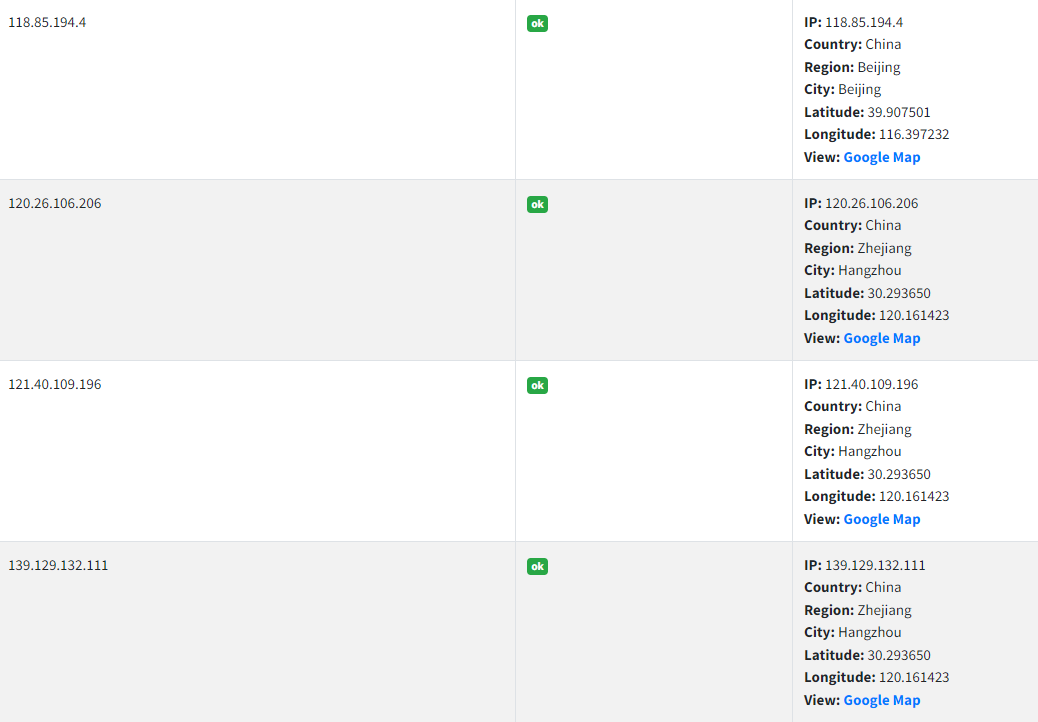
\includegraphics[width=1\textwidth]{./images/screenshot/NaughtyMaid/Domain1.png}
    \caption{Domain from MobSF 1}
    \label{fig:MaidDom1}
\end{figure}

\begin{figure}[h!]
\centering
    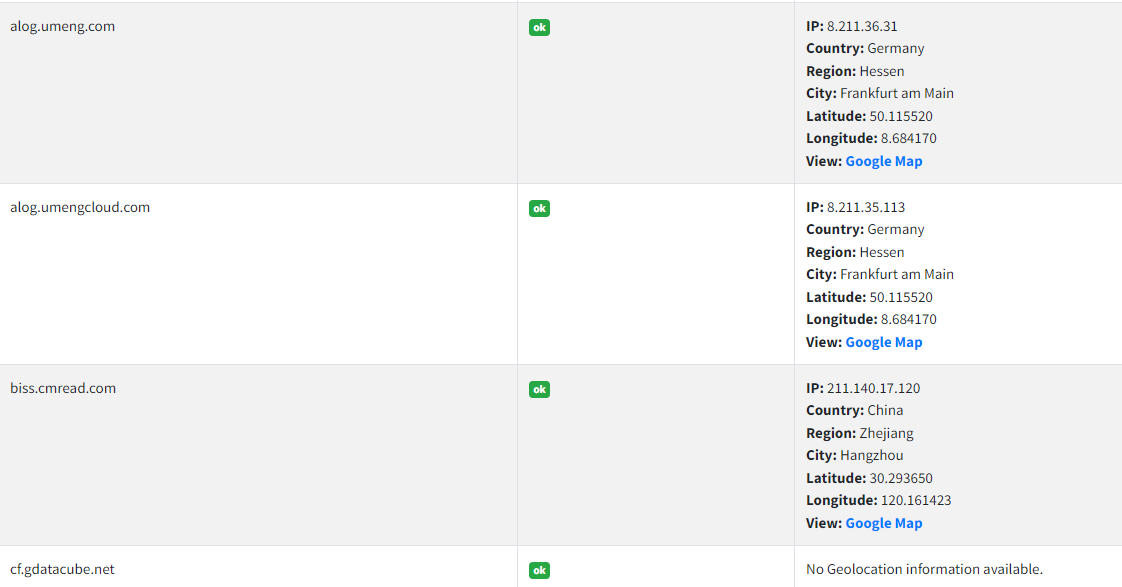
\includegraphics[width=1\textwidth]{./images/screenshot/NaughtyMaid/Domain2.png}
    \caption{Domain from MobSF 2}
    \label{fig:MaidDom2}
\end{figure}

\begin{figure}[h!]
\centering
    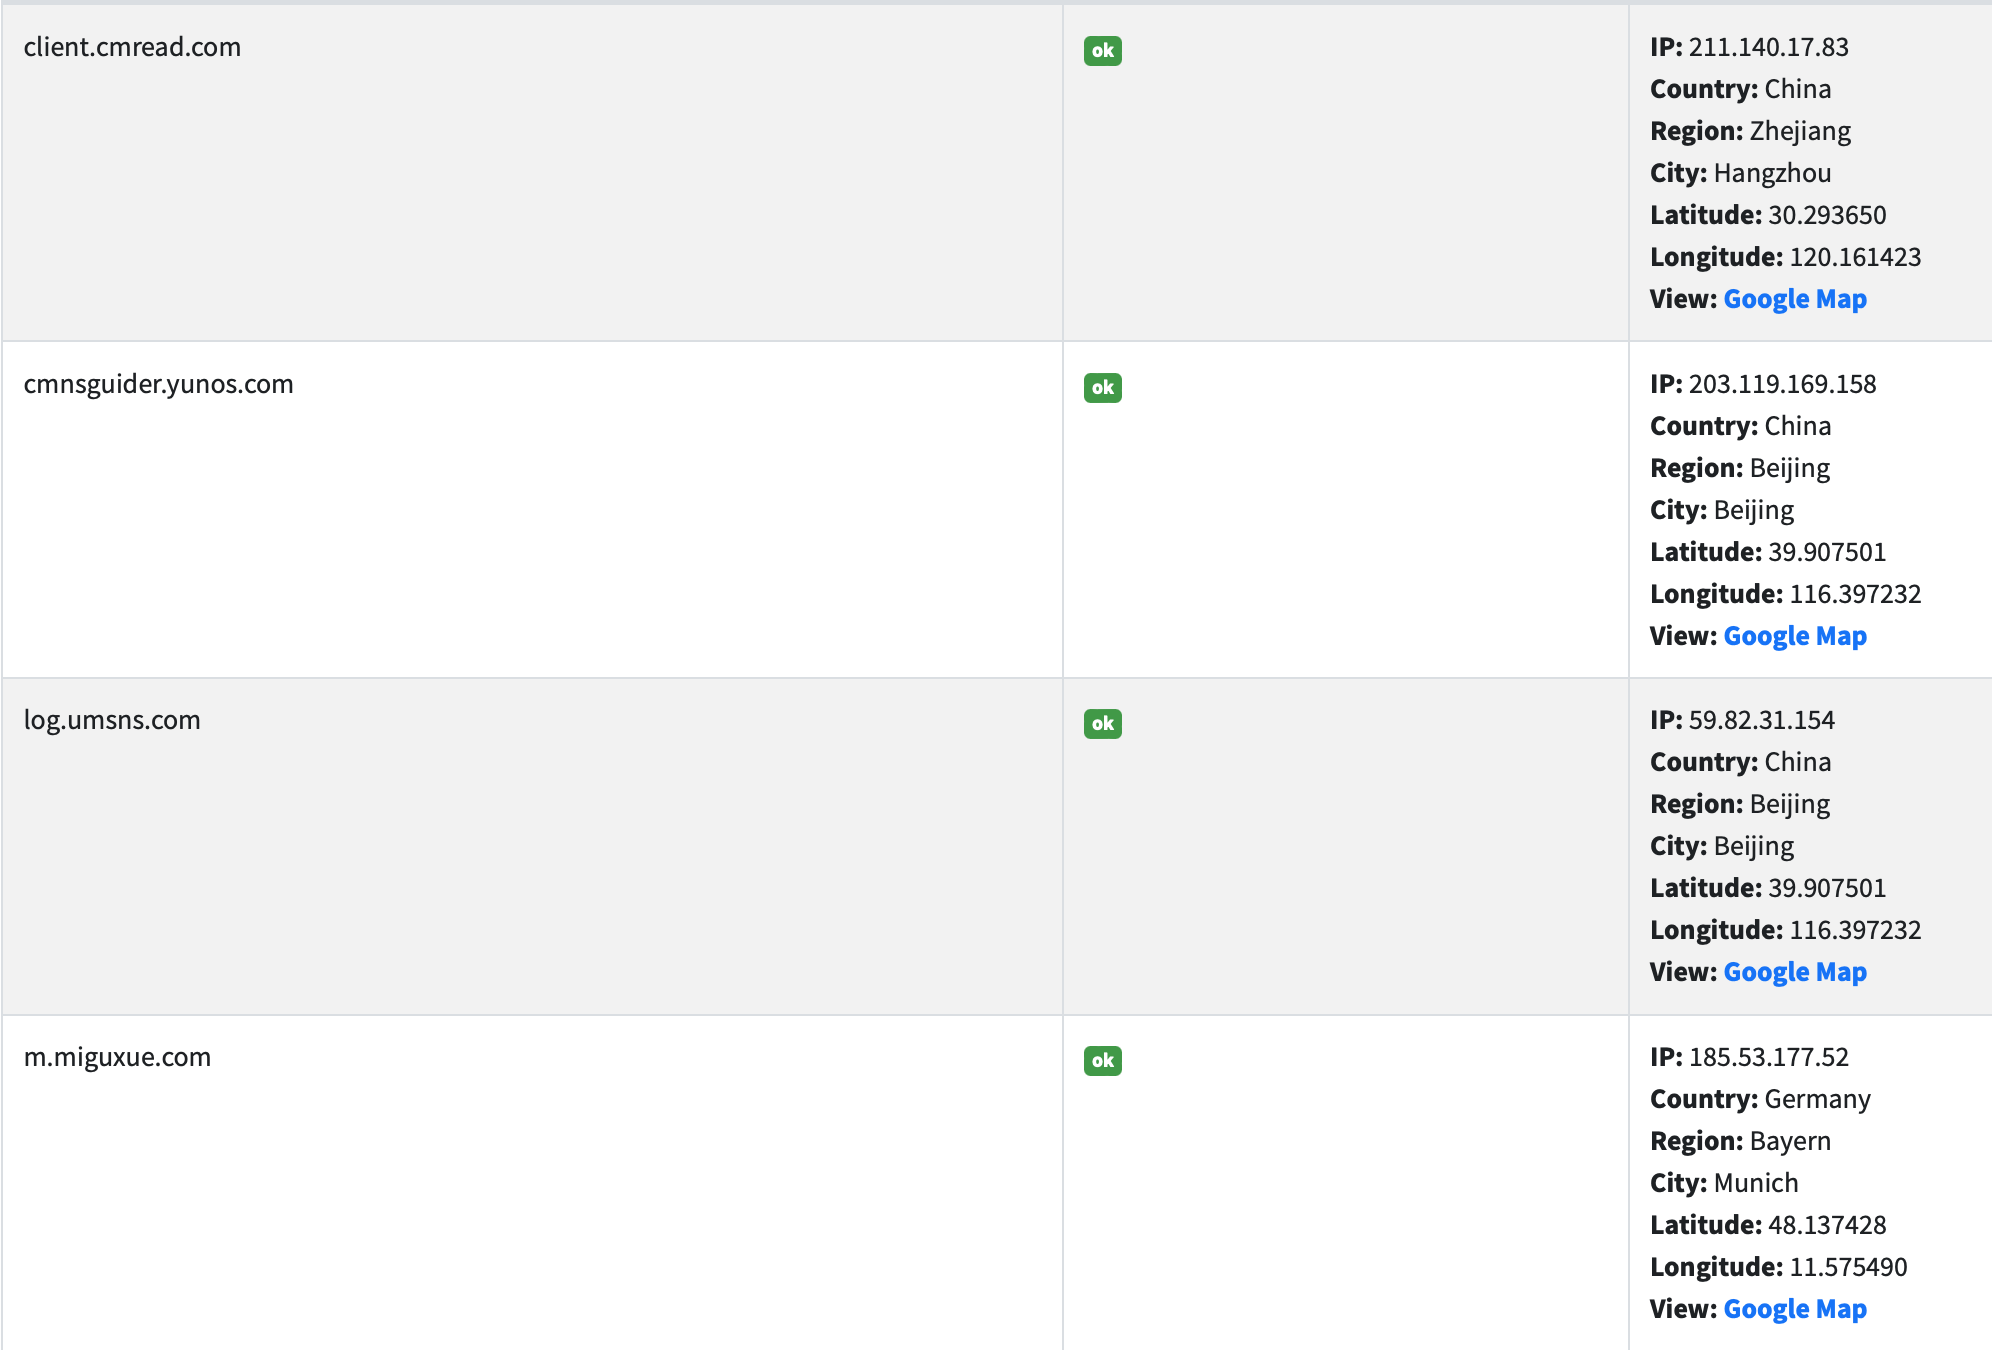
\includegraphics[width=1\textwidth]{./images/screenshot/NaughtyMaid/Domain3.png}
    \caption{Domain from MobSF 3}
    \label{fig:MaidDom3}
\end{figure}

\begin{figure}[h!]
\centering
    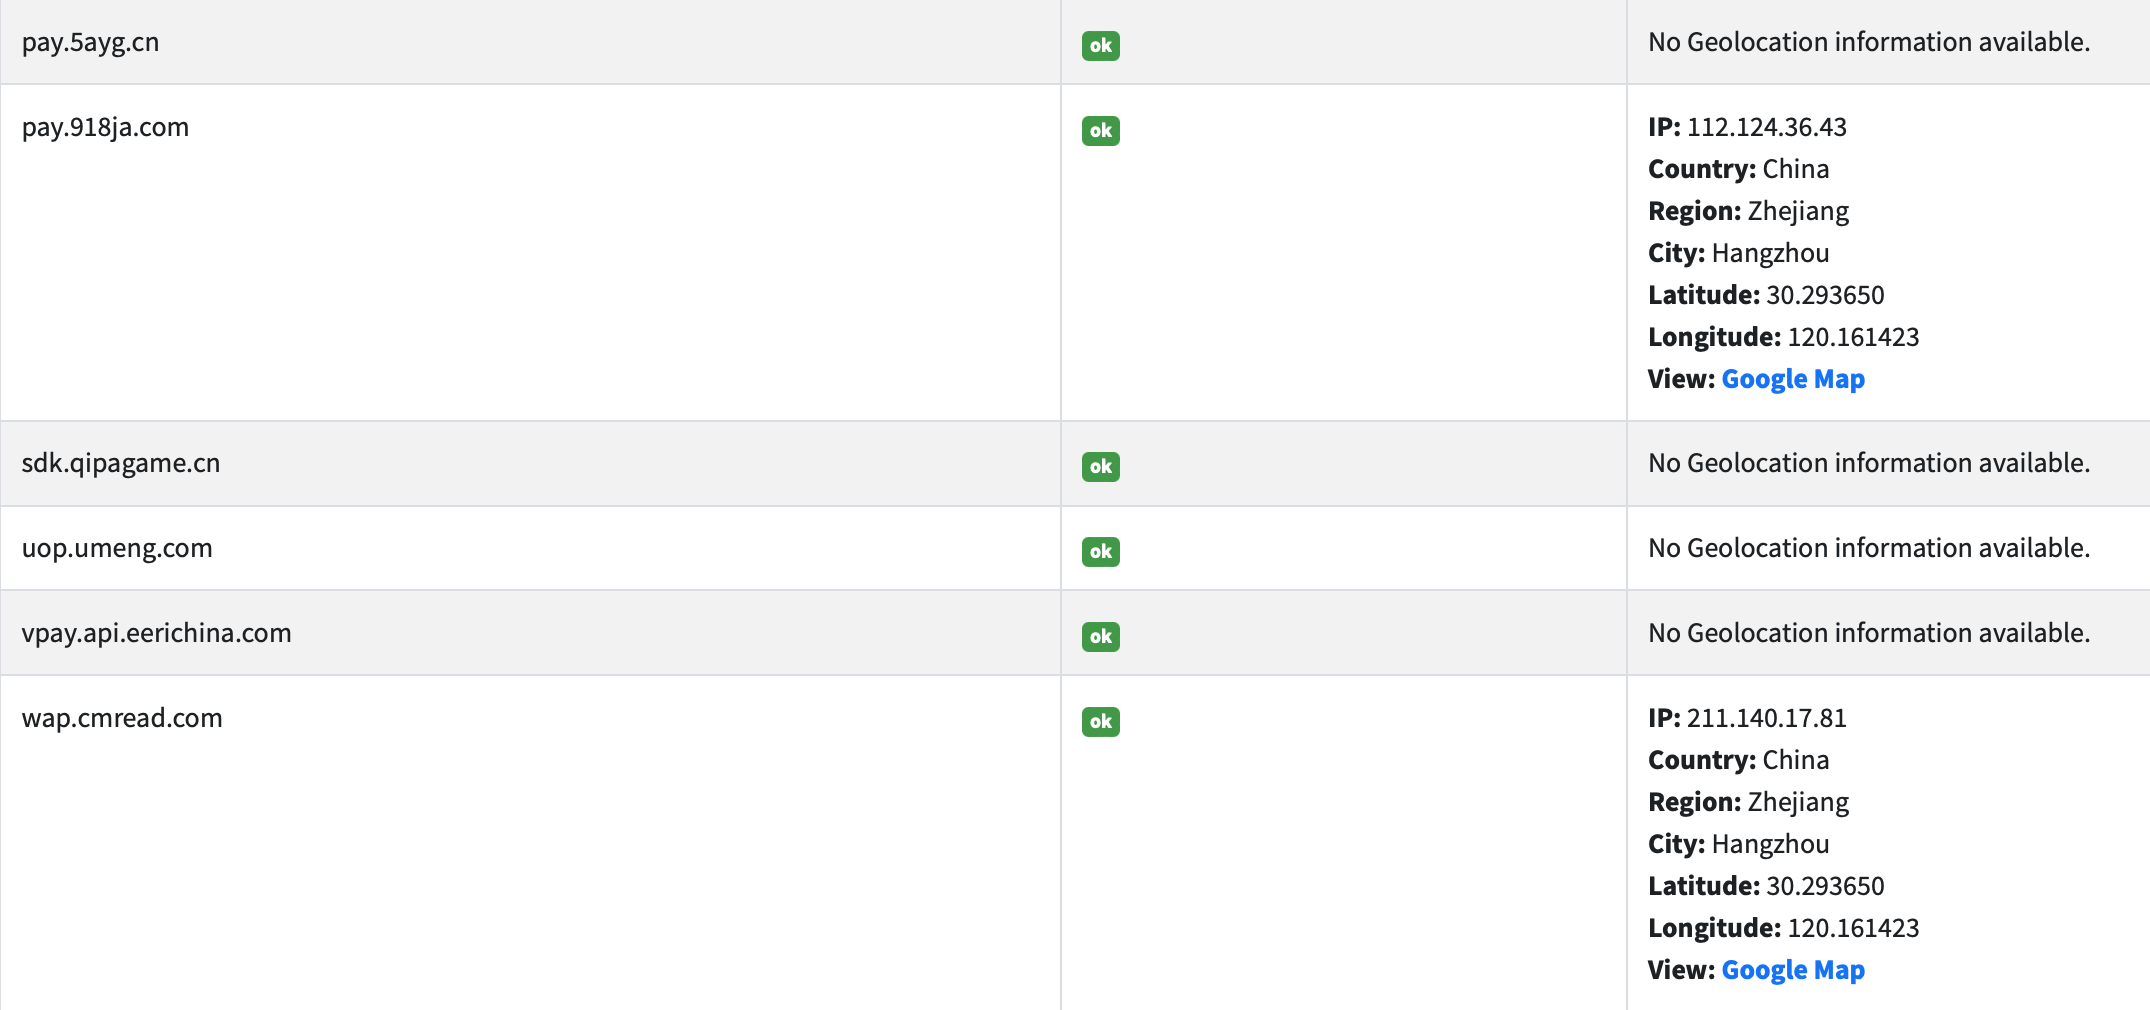
\includegraphics[width=1\textwidth]{./images/screenshot/NaughtyMaid/Domain4.png}
    \caption{Domain from MobSF 4}
    \label{fig:MaidDom4}
\end{figure}

\begin{figure}[h!]
\centering
    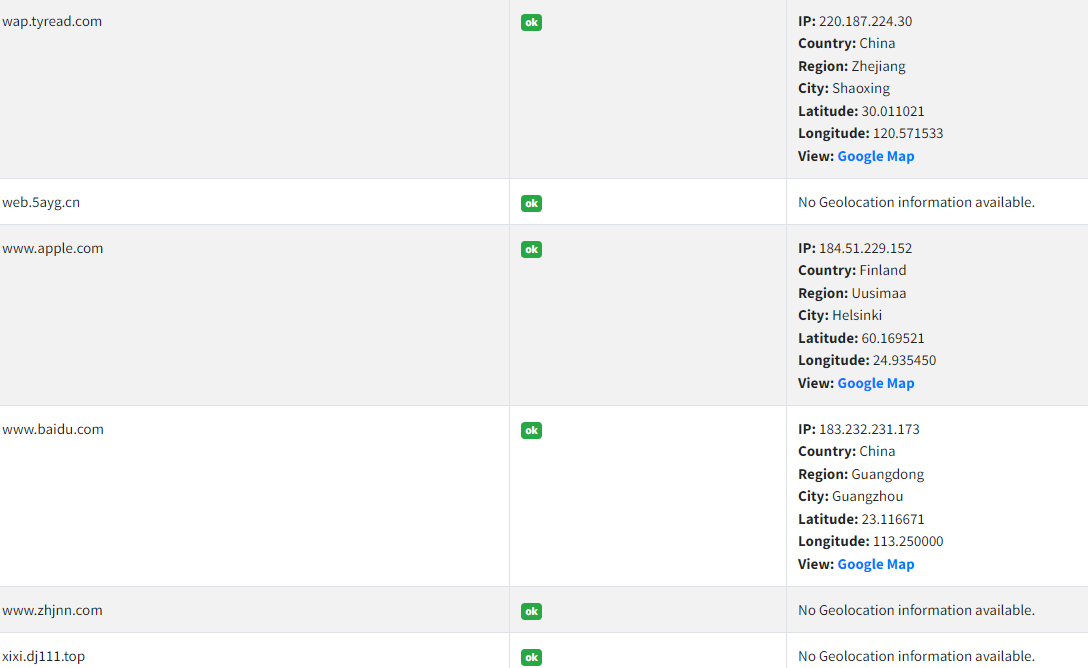
\includegraphics[width=1\textwidth]{./images/screenshot/NaughtyMaid/Domain5.png}
    \caption{Domain from MobSF 5}
    \label{fig:MaidDom5}
\end{figure}

In addition MobSF signal the presence of a tracker (Fig. \ref{fig:MaidTracker}) whose info can be consulted on exodus \footnote{\url{https://reports.exodus-privacy.eu.org/it/trackers/119/}}, in particular this tracker is associated with the \texttt{alog.umeng.com} domain present in Fig. \ref{fig:MaidDom2}

\begin{figure}[h!]
\centering
    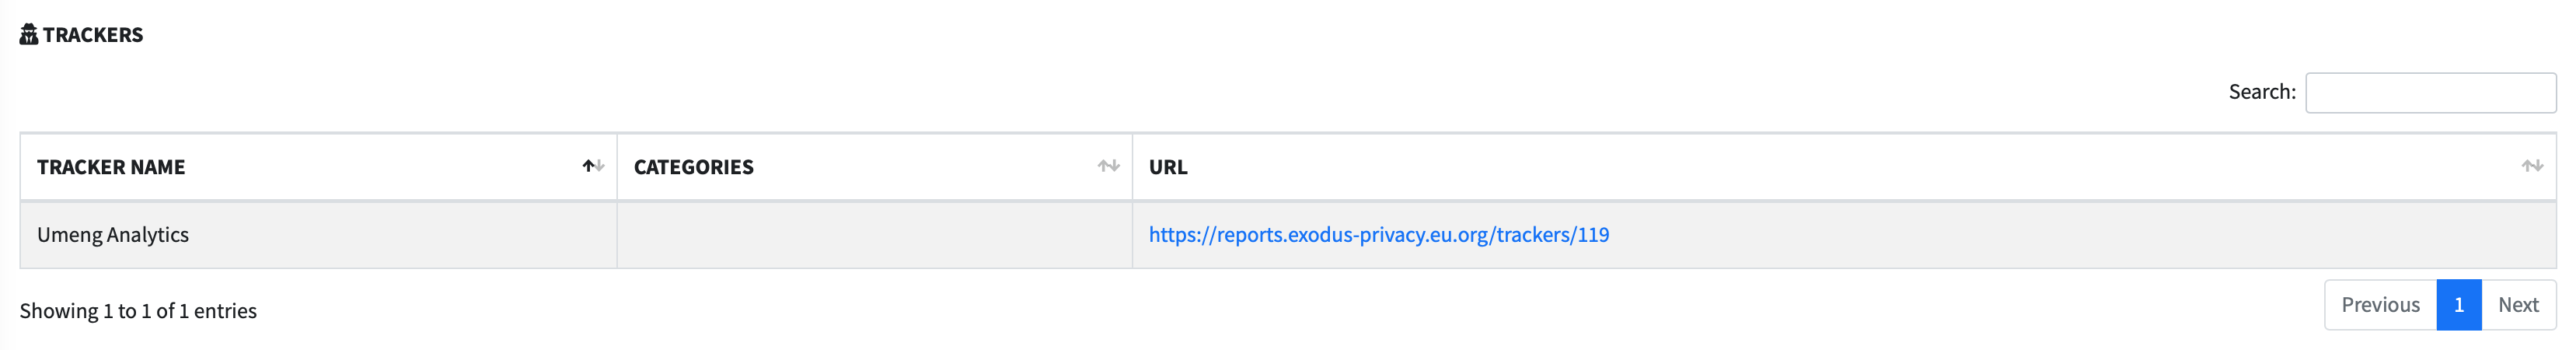
\includegraphics[width=1\textwidth]{./images/screenshot/NaughtyMaid/Tracker.png}
    \caption{Tracker signaled by MobSF}
    \label{fig:MaidTracker}
\end{figure}

\subsection{Code analysis}
As it can be seen in Fig. \ref{fig:CodeOrganization} the code is very obfuscated, since the classes do not contains significant names: most of them are a single character and there are lot of folders.
\begin{figure}[h!]
\centering
    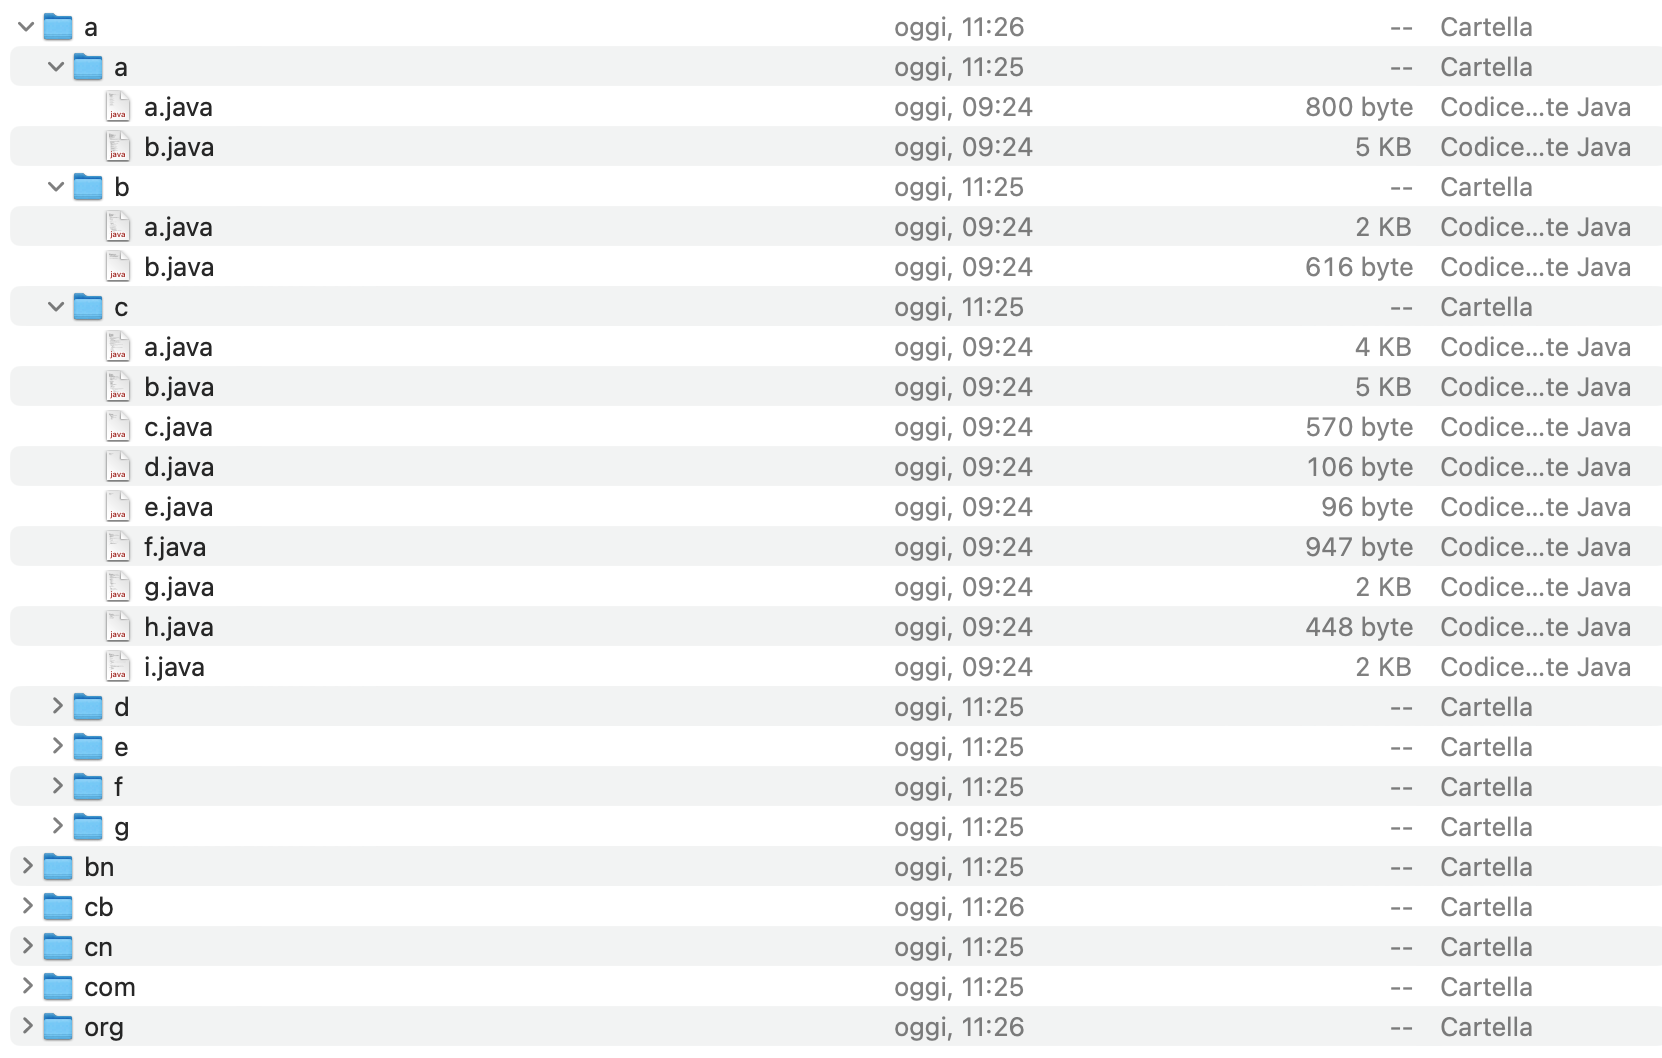
\includegraphics[width=1\textwidth]{./images/screenshot/NaughtyMaid/PackageStructure.png}
    \caption{Structure of the package}
    \label{fig:CodeOrganization}
\end{figure}
In addition the author also hides comments and valuable strings, with the class \\\texttt{com.mobile.bumptech.ordinary.miniSDK.SDK.a.a} (Fig.\ref{fig:loggerBase64}), which is basically a decryption function for text encrypted in base64 and xored with the value 66.
\begin{figure}[h!]
\centering
    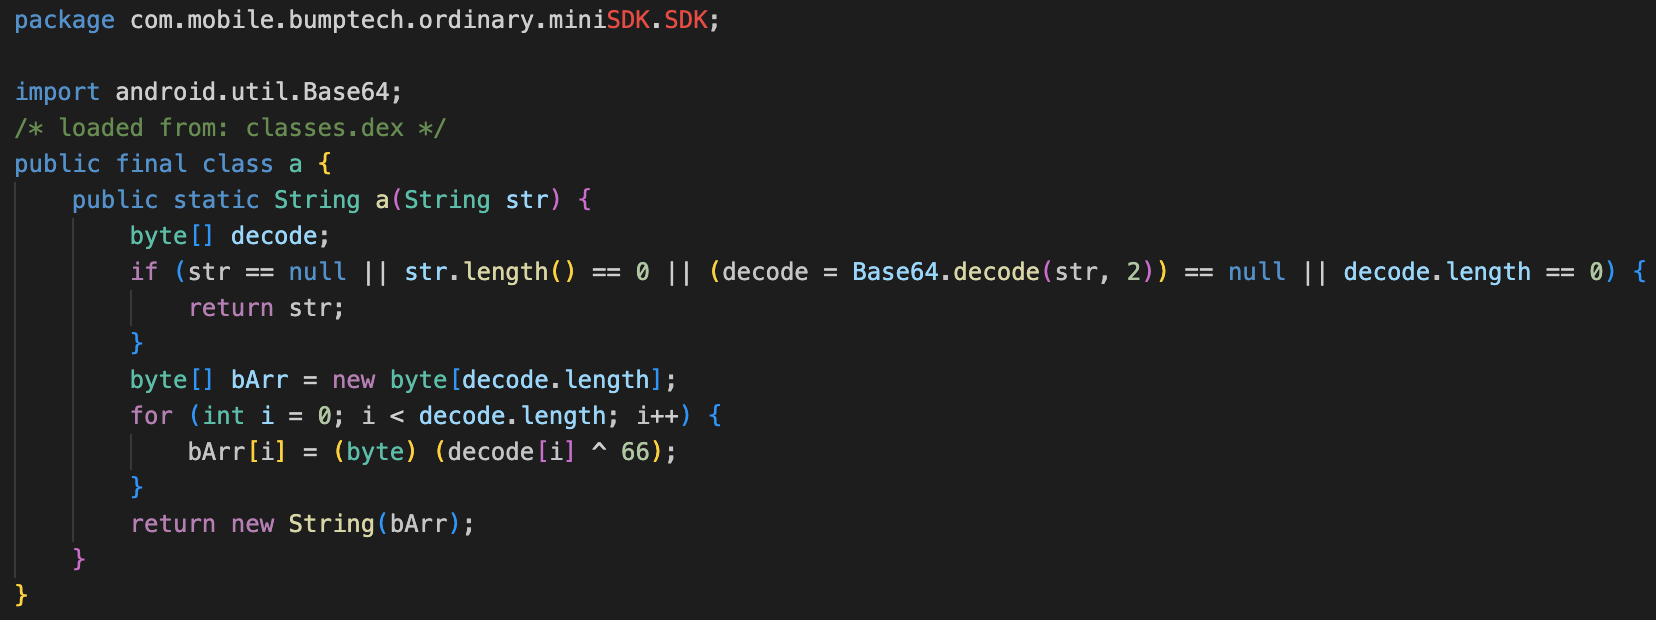
\includegraphics[width=1\textwidth]{./images/screenshot/NaughtyMaid/loggerBase64.png}
    \caption{com.mobile.bumptech.ordinary.miniSDK.SDK.a.a}
    \label{fig:loggerBase64}
\end{figure}
For better understanding the behavior, we decided to translate all "encrypted" base64 strings, and we show them in the Appendix (Chapter \ref{ch:Appendix}). \\
We also noticed that some classes seem to hide the malicious behavior, calling methods indirectly, like in the \texttt{MActivity} class. All methods of this class have the same structure, we show in Fig. \ref{fig:OnThouchEvent} \texttt{onTouchEvent}, it starts by calling \texttt{com.mobile.bumptech.ordinary.miniSDK.SDK.a.a}. Thanks to this solution, the author first obtains the method of the class and then invoke it, but text is not readable at first glance, making harder to understand what the application is doing. 
\begin{figure}[h!]
\centering
    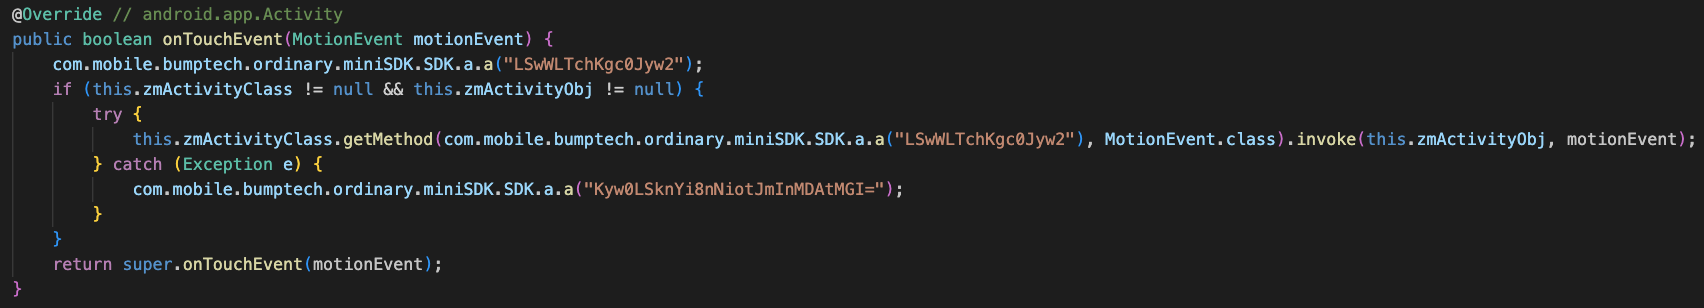
\includegraphics[width=1\textwidth]{./images/screenshot/NaughtyMaid/base64enc.png}
    \caption{MActivity: onTouchEvent}
    \label{fig:OnThouchEvent}
\end{figure}


Thanks to VirusTotal we were able to rapidly identify all activities, services and receivers started by the application which are listed in Fig. \ref{fig:activities} \ref{fig:services} \ref{fig:Receivers}
\begin{figure}[h!]
	\begin{subfigure}[h]{0.32\textwidth}
	    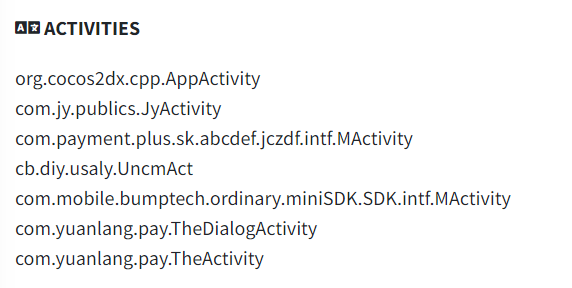
\includegraphics[width=1\textwidth]{./images/screenshot/NaughtyMaid/Activities.png}
	    \caption{Activities}
    		\label{fig:activities}
    \end{subfigure}
    \begin{subfigure}[h]{0.32\textwidth}
	    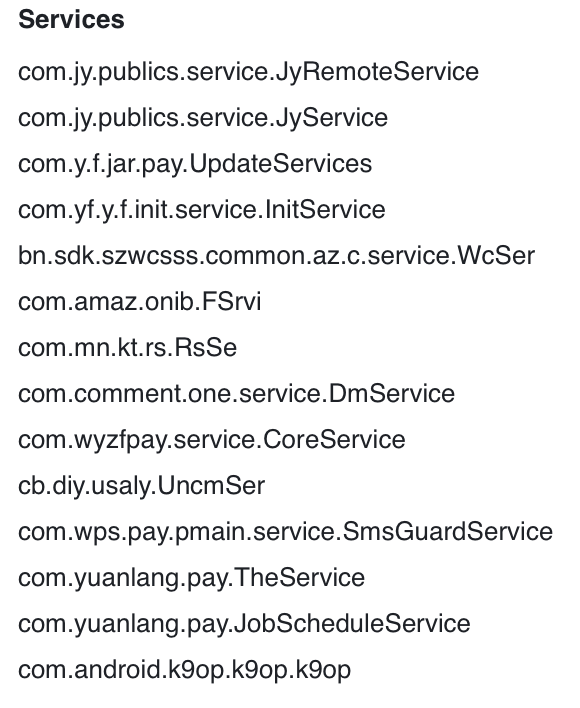
\includegraphics[width=1\textwidth]{./images/screenshot/NaughtyMaid/Services.png}
	    \caption{Services}
    		\label{fig:services}
    \end{subfigure}
    \begin{subfigure}[h]{0.32\textwidth}
	    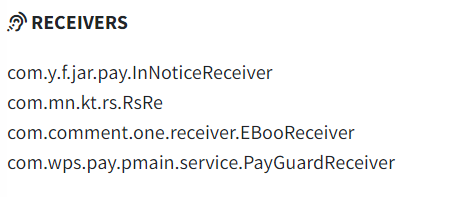
\includegraphics[width=1\textwidth]{./images/screenshot/NaughtyMaid/Receivers.png}
	    \caption{Receivers}
    		\label{fig:Receivers}
    \end{subfigure}
    \caption{Apps activities, services and receivers}
\end{figure}


\subsubsection{AppActivity}
The \texttt{AppActivity} class is the main entry point of the application, that is placed in the \texttt{org.cocos2dx.cpp} package. Cocos2d-x \footnote{\url{https://github.com/cocos2d/cocos2d-x}} is a multi-platform framework for building 2d games, interactive books, demos and other graphical applications. 
The class extends \texttt{Cocos2dxActivity} which extends Activity class of Android. When the activity is launched, the \texttt{onCreate} method is called. Firstly there is a check if the activity is the root of the task, if not, there is another check on the category of the intent, and if the \texttt{mainIntent} has a launcher category and the action of intent is main, the activity is stopped. The reason behind this behaviour might be related to an anti-debugging technique: the process asserts it being run from the launcher and if it senses it is a child process, maybe of a debugger, it stops its execution.

\begin{figure}[h!]
\centering
    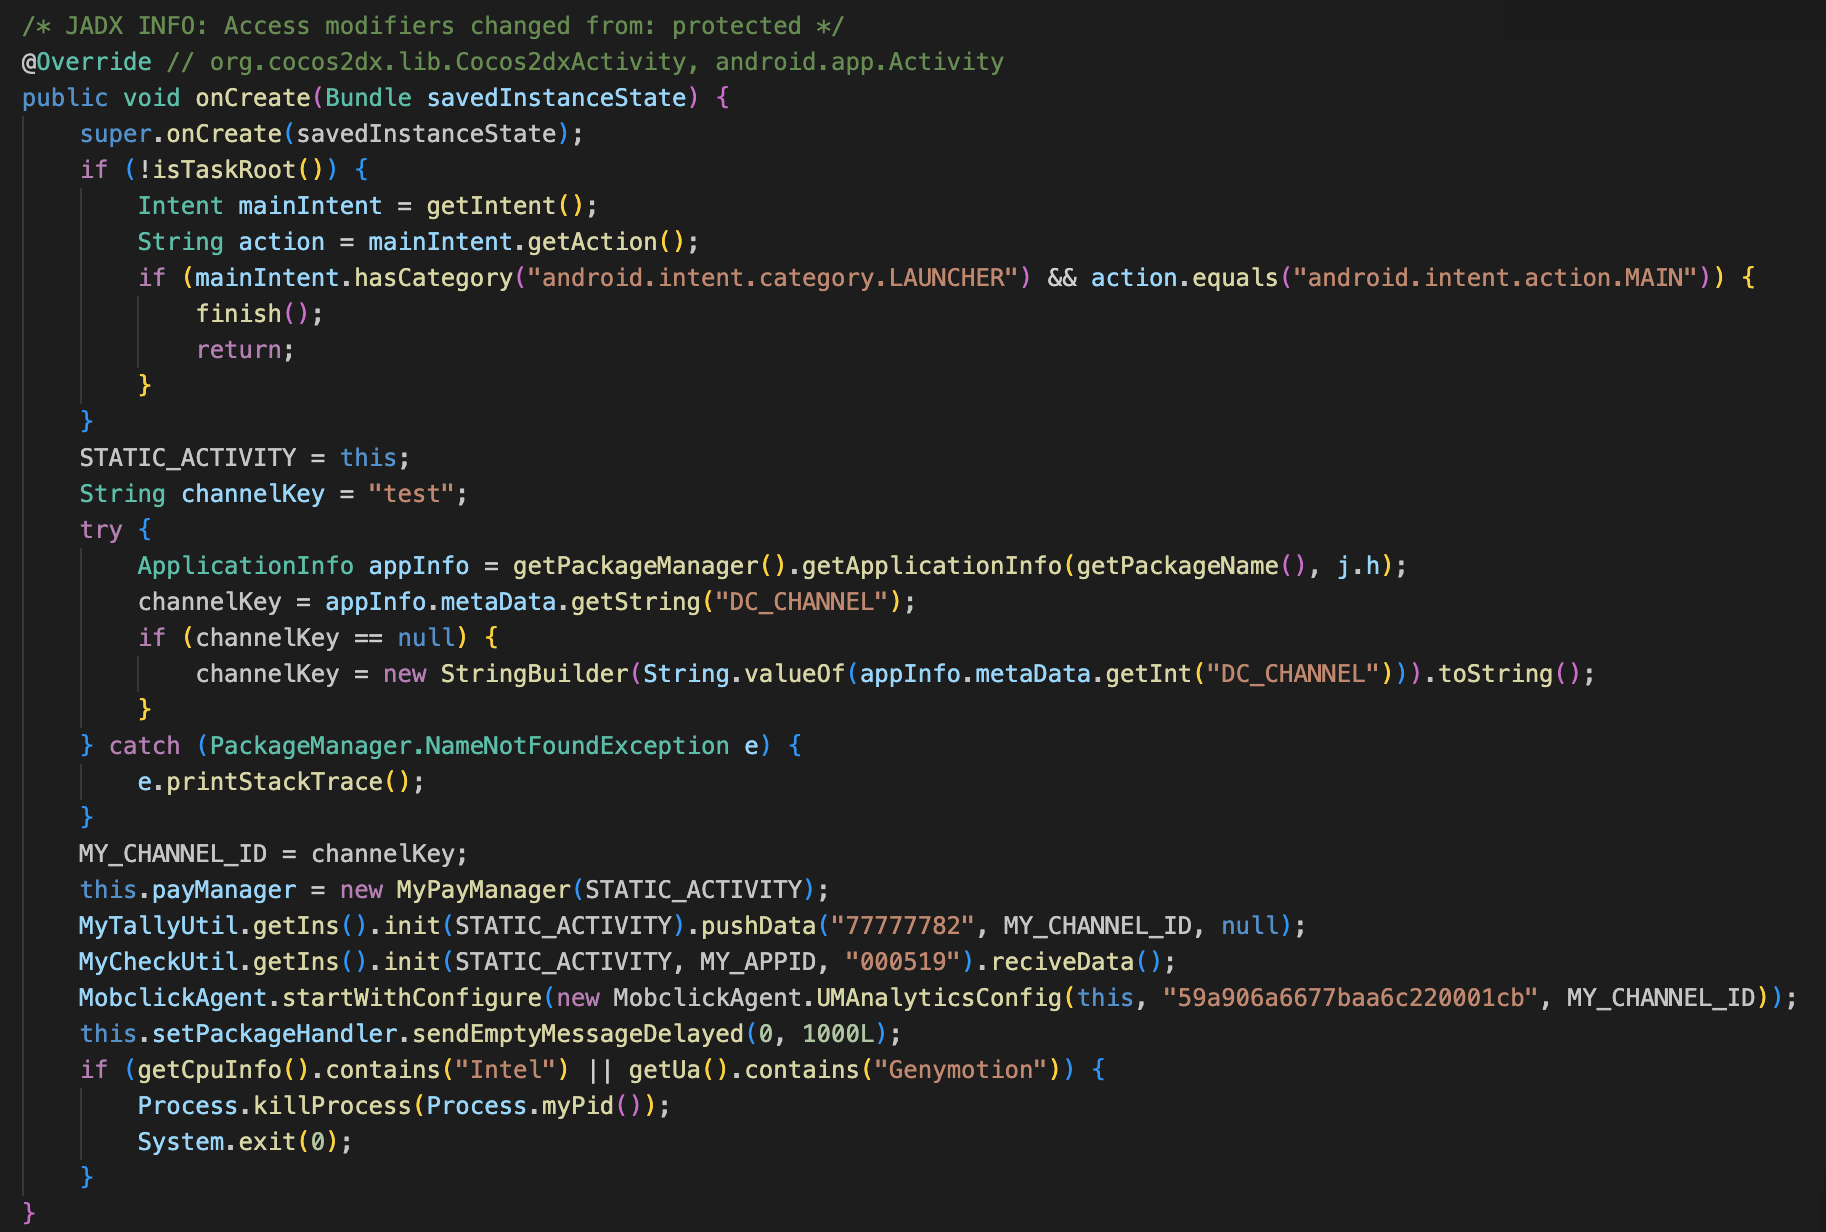
\includegraphics[width=1\textwidth]{./images/screenshot/NaughtyMaid/AppActivity.png}
    \caption{AppActivity:onCreate}
    \label{fig:AppActivityOnCreate}
\end{figure}

Then an object \texttt{MyPayManager} is created and the init method of \texttt{MyTallyUtil} and \texttt{MyCheckUtil} are called. At the end of the method there is also an interesting behavior, there is a check against the name of the CPU, with \texttt{getCPUInfo()} (Fig \ref{fig:AppActivitygetCPUInfo}) and the manifacturer, with \texttt{getUa()} (Fig \ref{fig:AppActivitygetUa}). \texttt{getCPUInfo()} basically executes the command "cat /proc/cpuinfo", while \texttt{getUa()} gets information of the model, the manifacturer and the brand. If the cpu string contains "Intel" or the manifacturer string contains "Genymotion" the activity kills the current process. This is likely a protection measure that the author inserts, so that the app can't run on a virtual environment. 
\begin{figure}[h!]
\centering
    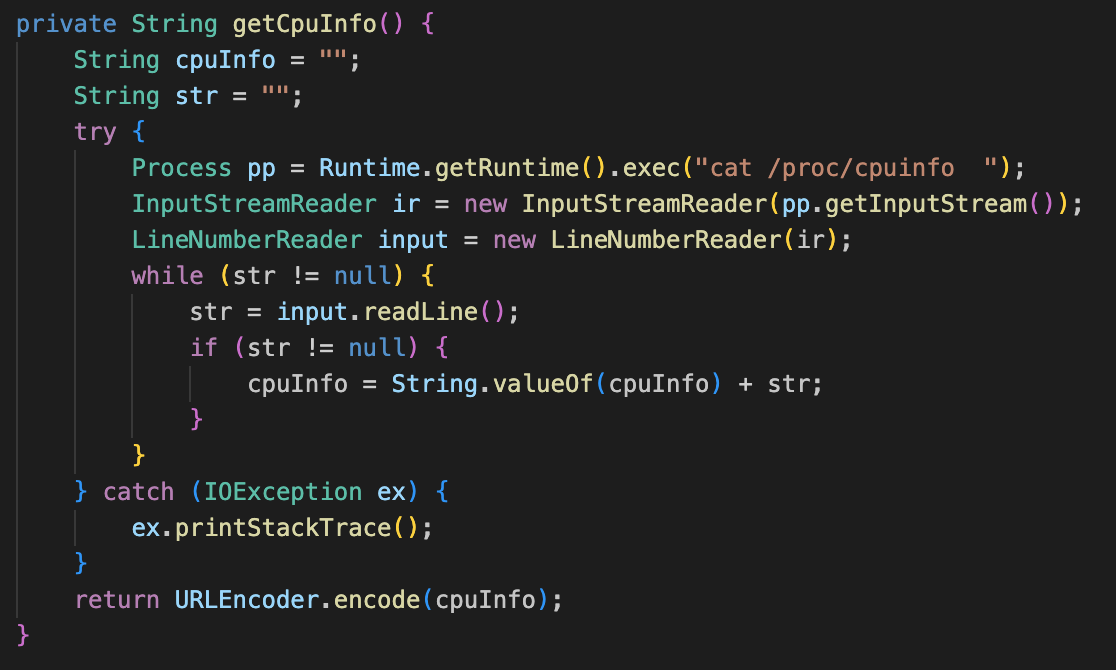
\includegraphics[width=1\textwidth]{./images/screenshot/NaughtyMaid/getCPUinfo.png}
    \caption{AppActivity:getCPUInfo}
    \label{fig:AppActivitygetCPUInfo}
\end{figure}
\begin{figure}[h!]
\centering
    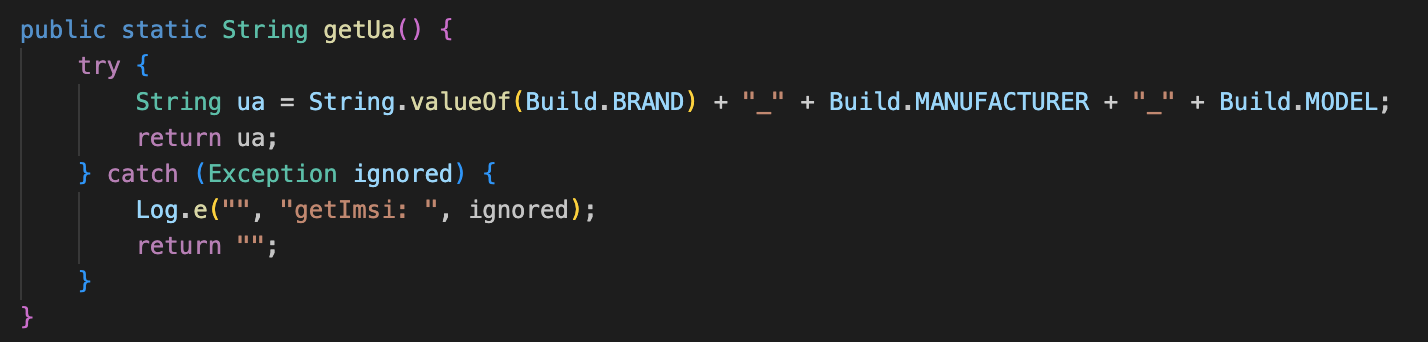
\includegraphics[width=1\textwidth]{./images/screenshot/NaughtyMaid/getUa.png}
    \caption{AppActivity:getUa}
    \label{fig:AppActivitygetUa}
\end{figure}

\subsubsection{myPayManager}
The flow of the program than moves to the \texttt{MyPayManager} class Fig. \ref{fig:myPayManager} where a list of paid services is instantiated and then added to a list of messages; in addition each service implements the interface \texttt{IPayHelper} and defines its own \texttt{usePay()} method, this allows the malicious app to fire all paid services with a single for loop. It is important to point out that each service is different from the others  so, given that they all implement malicious behaviors, for the sake of brevity we decided to show a single one of them. 
\begin{figure}[h!]
\centering
    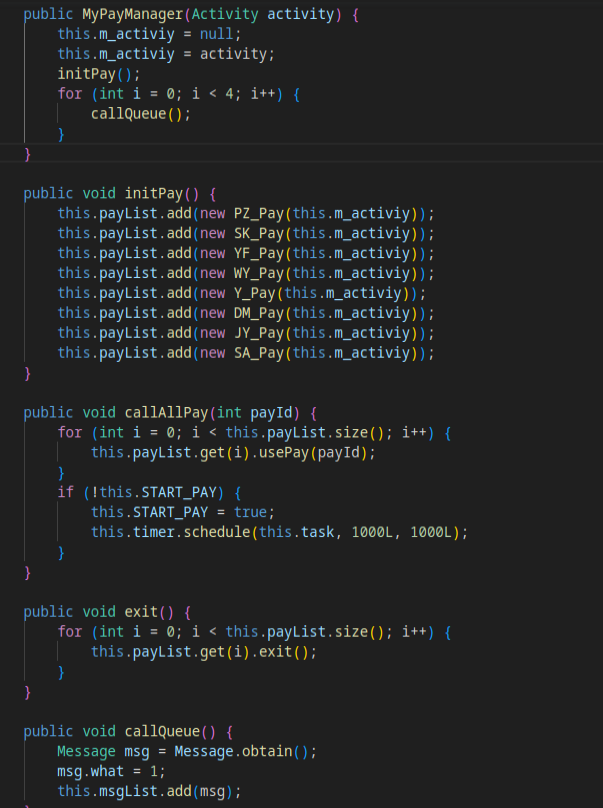
\includegraphics[width=0.8\textwidth]{./images/screenshot/NaughtyMaid/myPayManager.png}
    \caption{myPayManager}
    \label{fig:myPayManager}
\end{figure}

\begin{figure}[h!]
\centering
    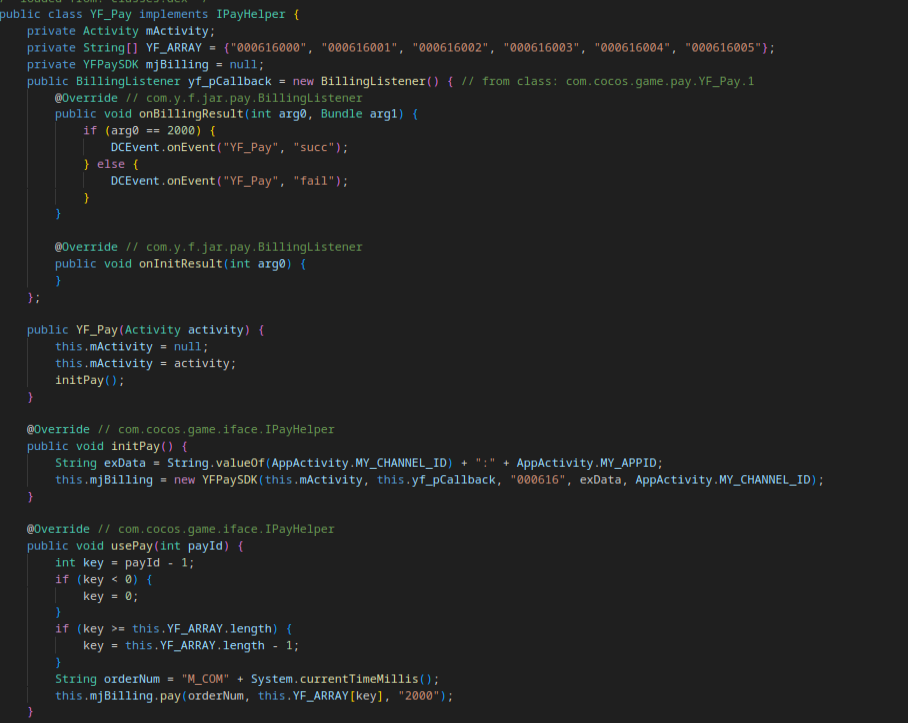
\includegraphics[width=1\textwidth]{./images/screenshot/NaughtyMaid/YFPay.png}
    \caption{YF\_Pay}
    \label{fig:YFPay}
\end{figure}

\begin{figure}[h!]
\centering
    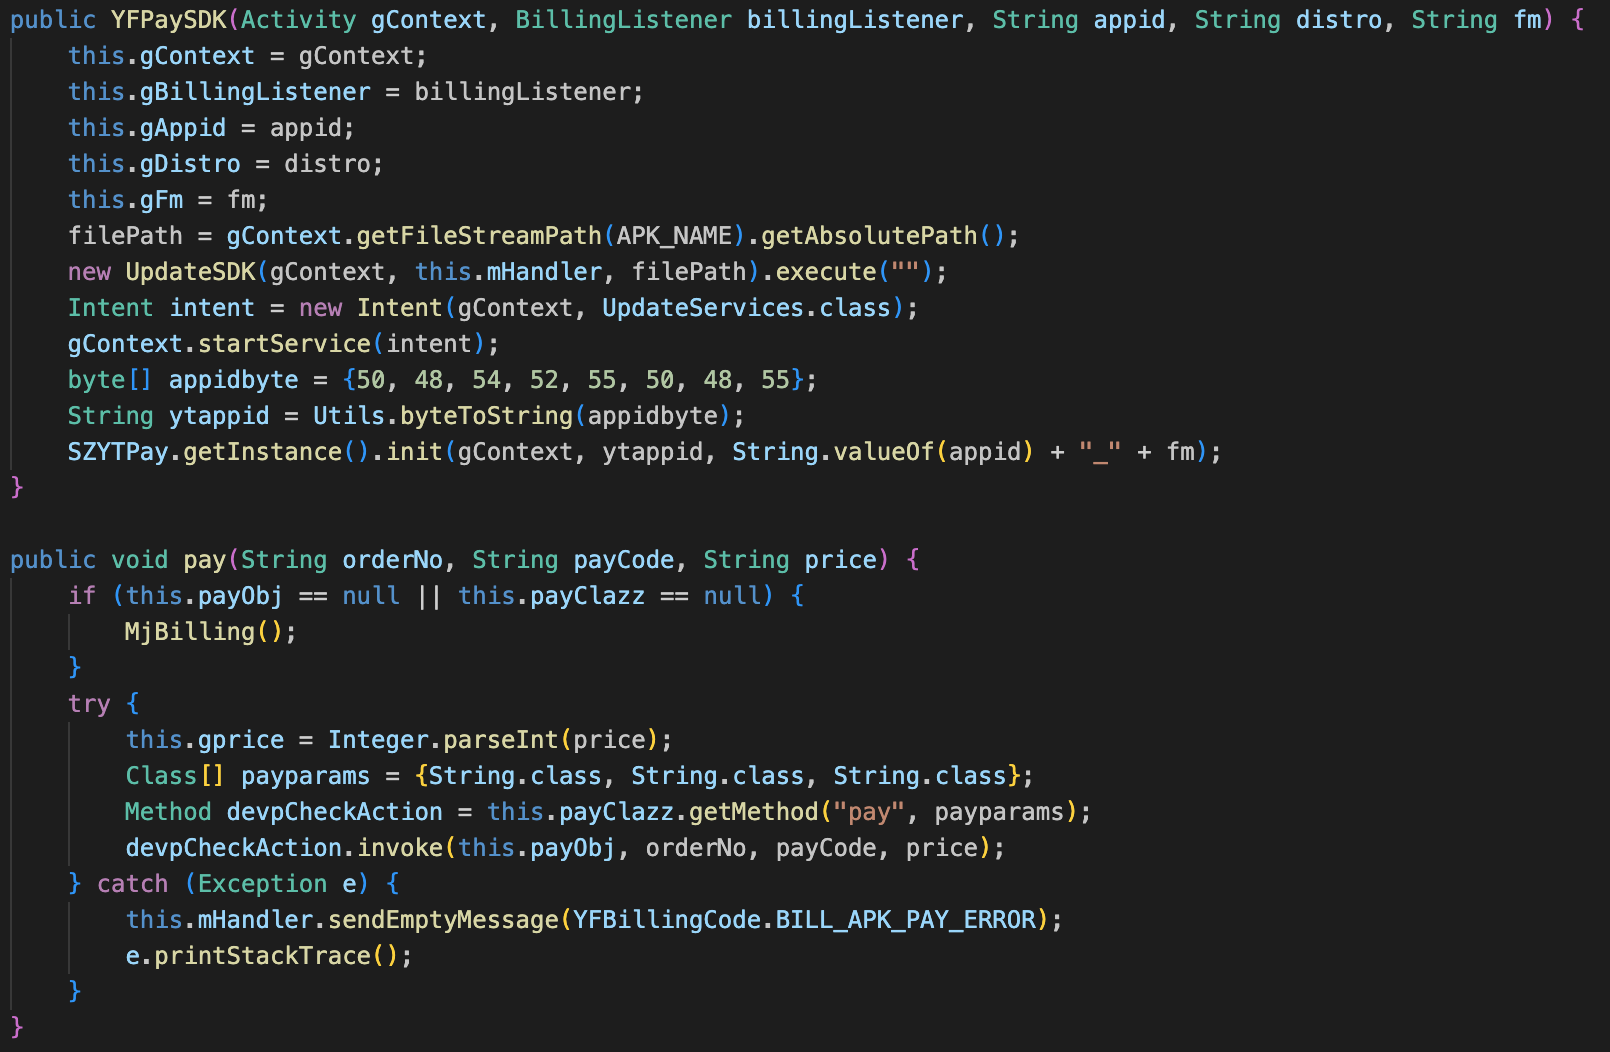
\includegraphics[width=1\textwidth]{./images/screenshot/NaughtyMaid/YFPaySDK.png}
    \caption{YFPaySDK}
    \label{fig:YFPaySDK}
\end{figure}

\begin{figure}[h!]
\centering
    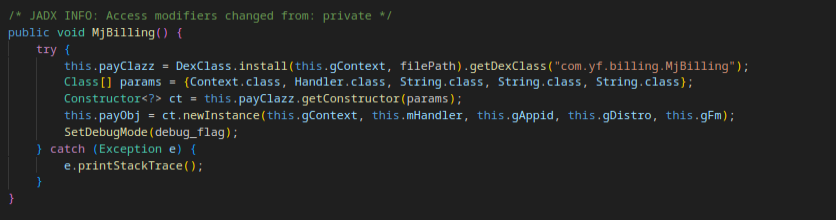
\includegraphics[width=1\textwidth]{./images/screenshot/NaughtyMaid/MjBilling.png}
    \caption{MjBilling}
    \label{fig:MjBilling}
\end{figure}


In particular the class chosen is \texttt{YF\_Pay} (Fig. \ref{fig:YFPay}) since it is the most articulated and, as it can be seen in the picture, it calls the constructor for \texttt{YFPaySDK} Fig. \ref{fig:YFPaySDK}; after some initialization steps it starts \texttt{UpdateServices}, which installs an apk that at first sight was not found in the archive we received. After a meticulous research in the codebase we identify a method that loads \texttt{yf.conf} encoded in base64 (Fig. \ref{fig:UpdateSDKcpFile}), and then uses it as an apk. This is not the only file we discovered, hidden in this manner, and it is of course another proof that obfuscation of malicious behavior is used throughout the project. In this specific case the method \texttt{MjBilling()}  is loaded via \texttt{DexClass} (Fig. \ref{fig:MjBilling}). We decompiled the resulting apk and we found all sources show in Fig. \ref{fig:YFconf}

\begin{figure}[h!]
\centering
    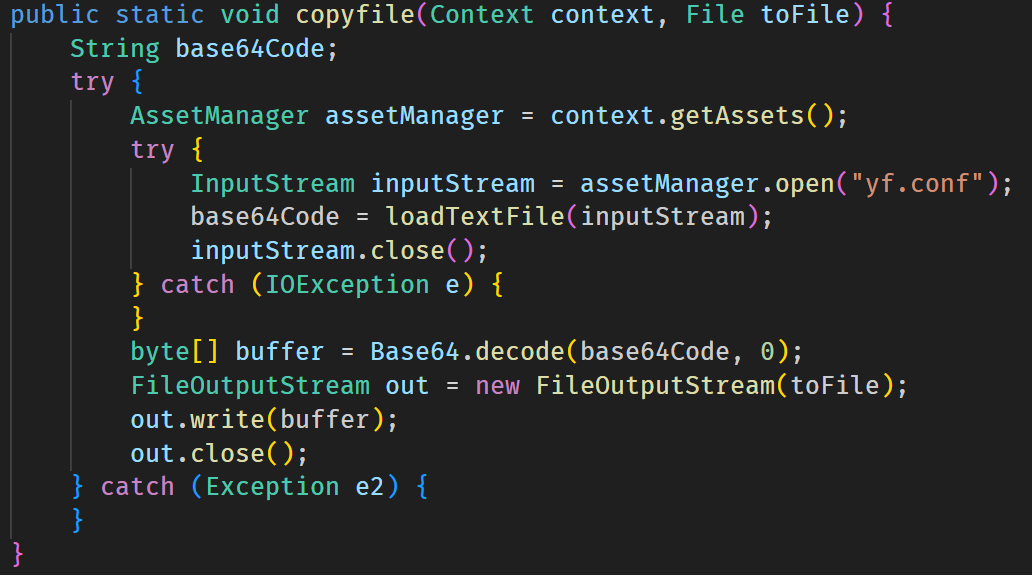
\includegraphics[width=1\textwidth]{./images/screenshot/NaughtyMaid/YFDecode.png}
    \caption{UpdateSDK: copyFile()}
    \label{fig:UpdateSDKcpFile}
\end{figure}

\begin{figure}[h!]
\centering
    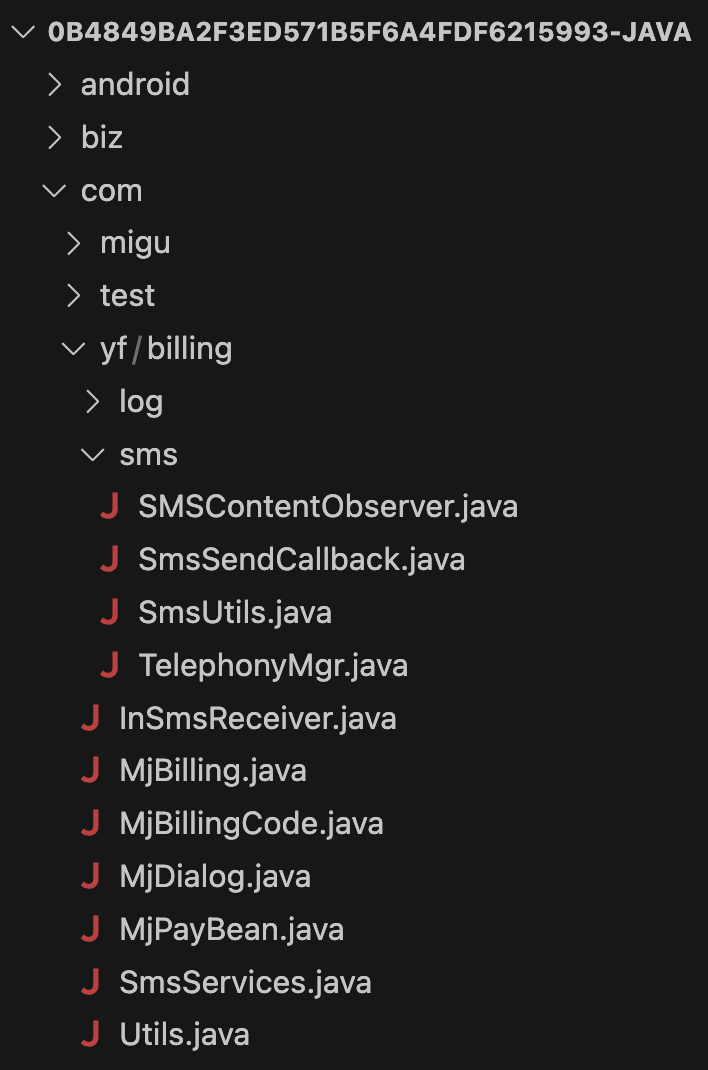
\includegraphics[width=0.6\textwidth]{./images/screenshot/NaughtyMaid/YFconf.png}
    \caption{YF.conf structure}
    \label{fig:YFconf}
\end{figure}

\subsubsection{Receiver}
Before executing the pay method however the program creates a new intent with the \texttt{UpdateService} class Fig. \ref{fig:UpdateService} that installs in the \texttt{initSmsService} method a class from the dex file. Similarly the \texttt{InNoticeReceiver} Fig. \ref{fig:InNoticeReceiver} acts as a receiver and installs a class from the dex file too.

\begin{figure}[h!]
\centering
    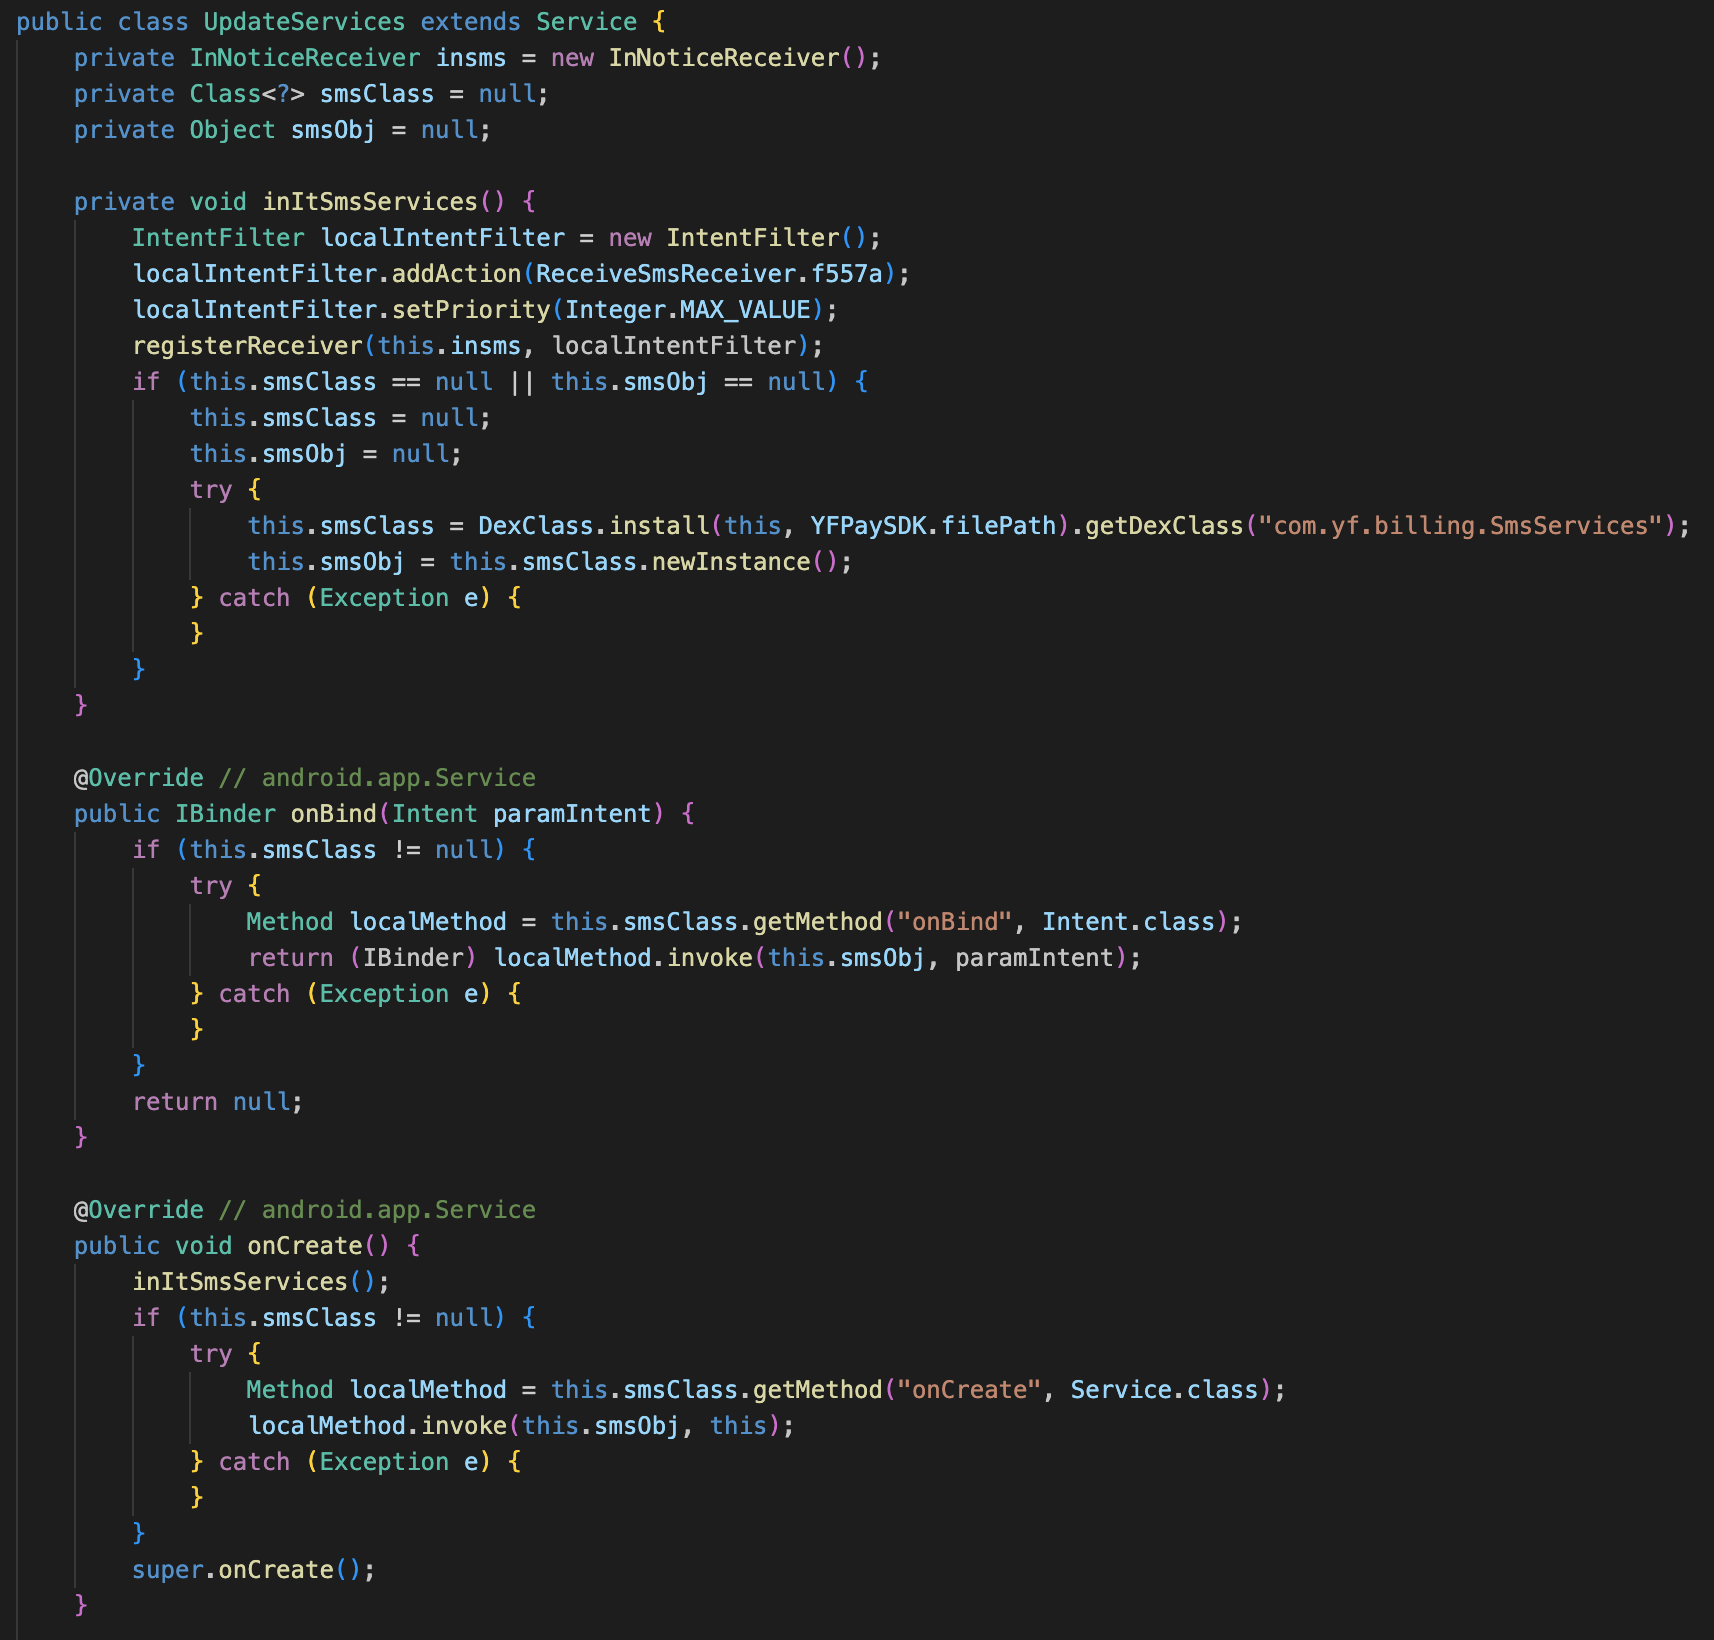
\includegraphics[width=1\textwidth]{./images/screenshot/NaughtyMaid/UpdateService.png}
    \caption{UpdateService}
    \label{fig:UpdateService}
\end{figure}

\begin{figure}[h!]
\centering
    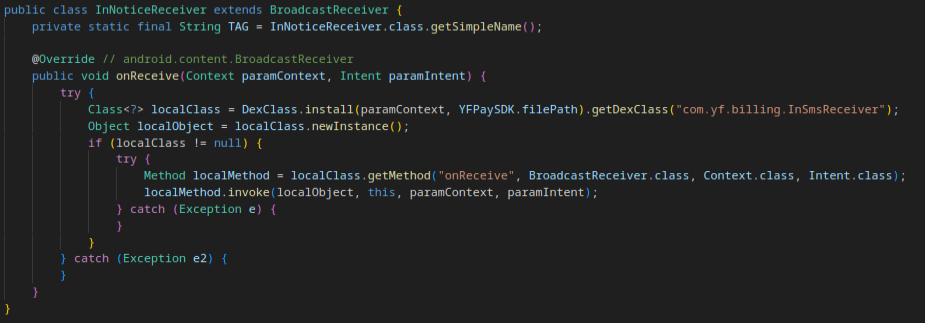
\includegraphics[width=1\textwidth]{./images/screenshot/NaughtyMaid/InNoticeReceiver.png}
    \caption{InNoticeReceiver}
    \label{fig:InNoticeReceiver}
\end{figure}

\subsubsection{SZYTPay}
After the UpdateService, the SZYTPay class is used (Fig \ref{fig:SZYTPay}) which calls the \texttt{SdkDlm} class to install plugins of possible malicious intent (Fig. \ref{fig:SZYTPay2}).
\begin{figure}[h!]
\centering
    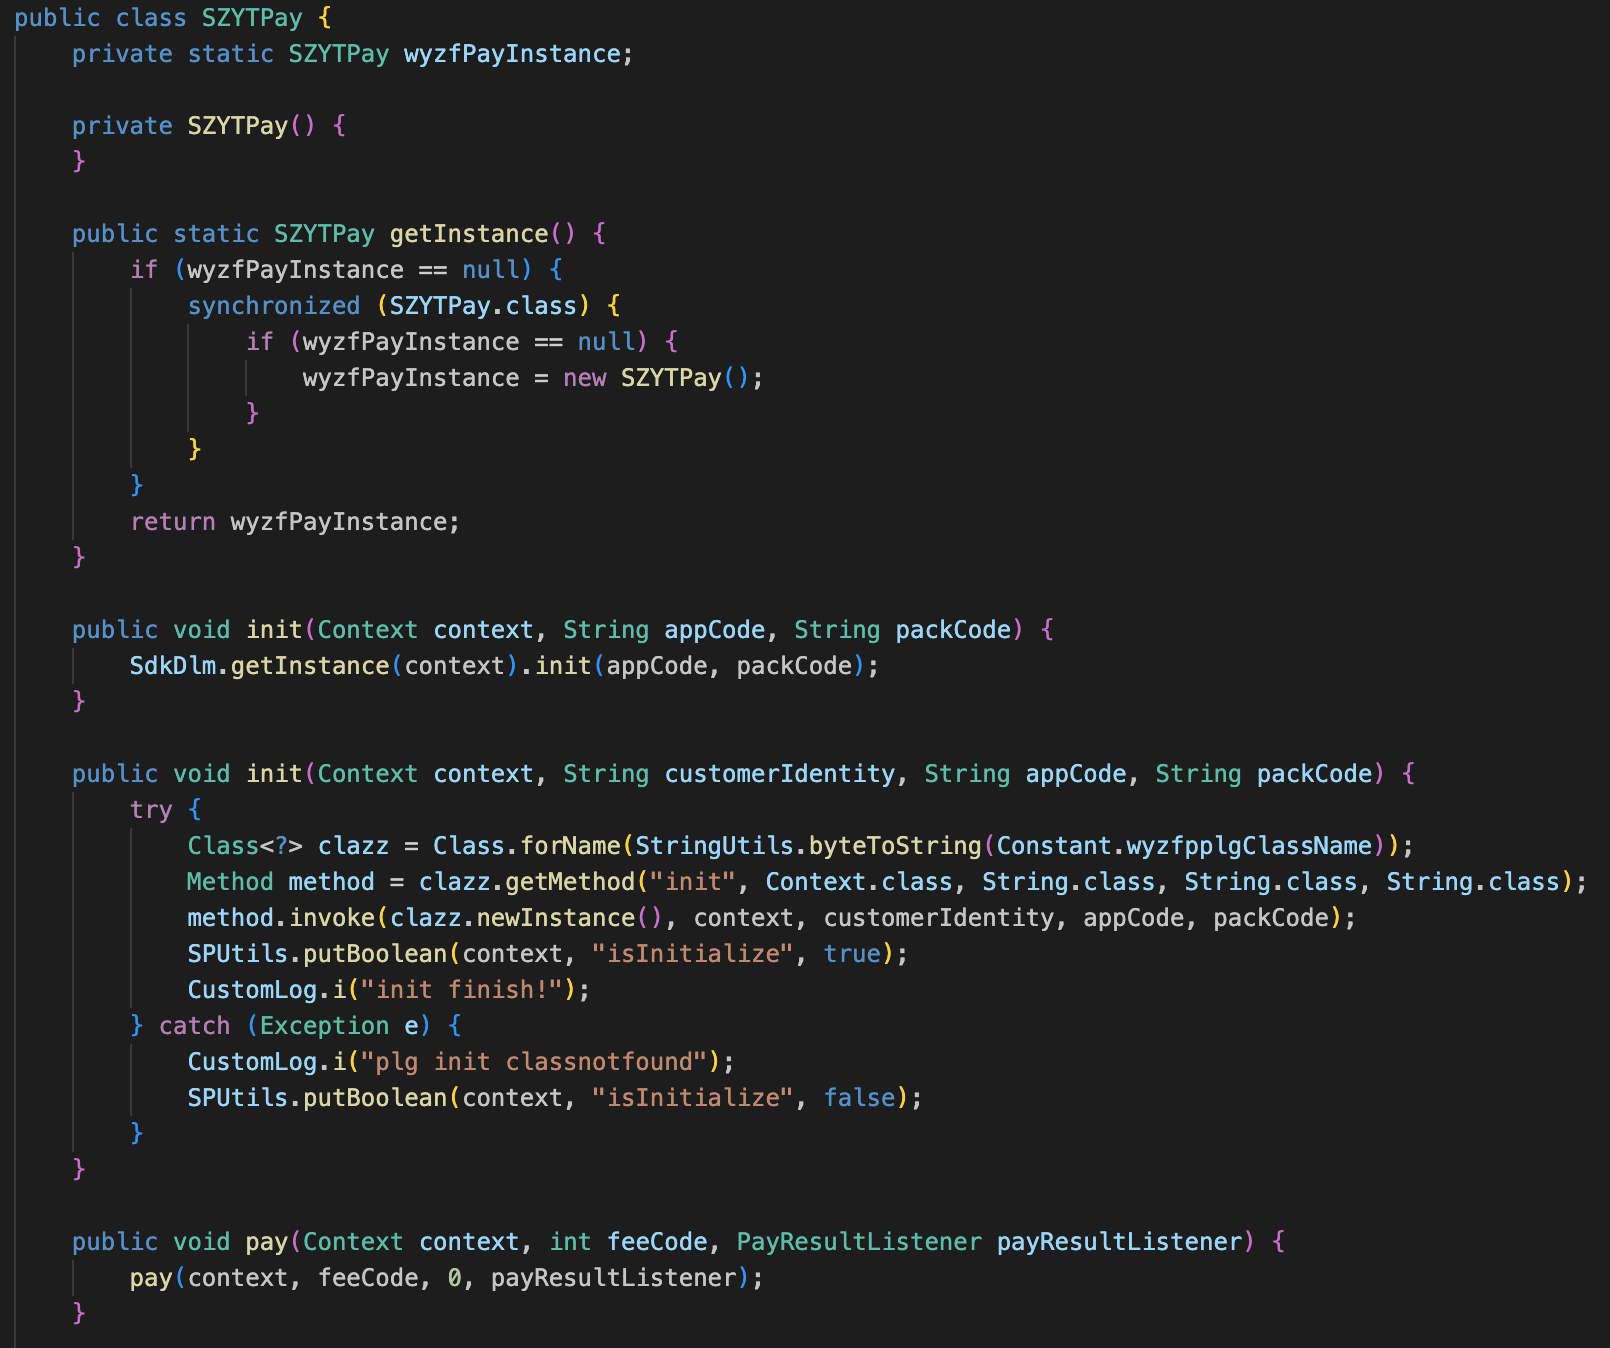
\includegraphics[width=1\textwidth]{./images/screenshot/NaughtyMaid/SZYPay.png}
    \caption{SZYTPay}
    \label{fig:SZYTPay}
\end{figure}

\begin{figure}[h!]
\centering
    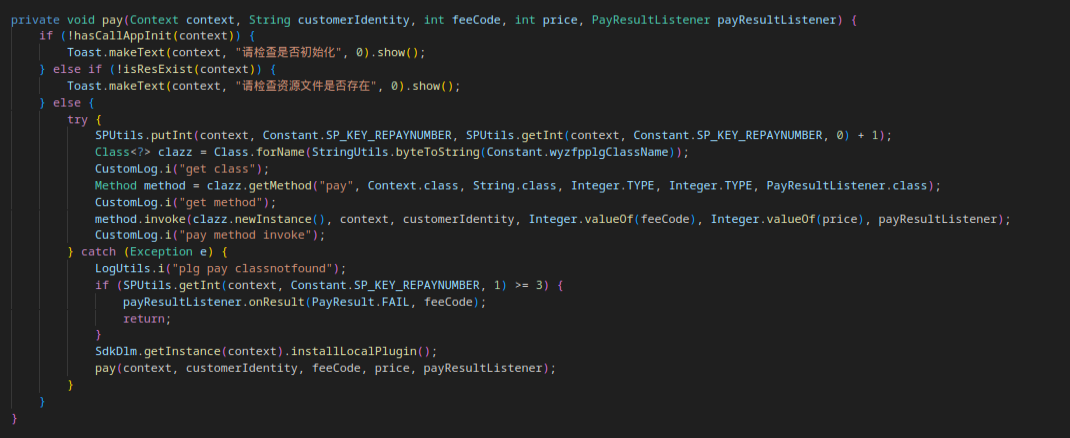
\includegraphics[width=1\textwidth]{./images/screenshot/NaughtyMaid/SZYPay2.png}
    \caption{SZYTPay pay method}
    \label{fig:SZYTPay2}
\end{figure}

In general what we can say is that the malware creates a number of paid services related to SMS fraud and is also able to install new plugins.
As further proof of malicious activities related to the SMS handling in the obfuscated code there is a call to a method used for deleting incoming SMS messages so that the phone owner would not notice any strange behavior. Fig. \ref{fig:DeleteSMS} and \ref{fig:CDO}.

\begin{figure}[h!]
\centering
    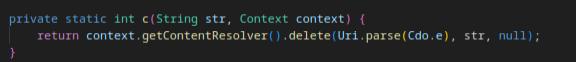
\includegraphics[width=1\textwidth]{./images/screenshot/NaughtyMaid/DeleteSMS.png}
    \caption{DeleteSMS}
    \label{fig:DeleteSMS}
\end{figure}

\begin{figure}[h!]
\centering
    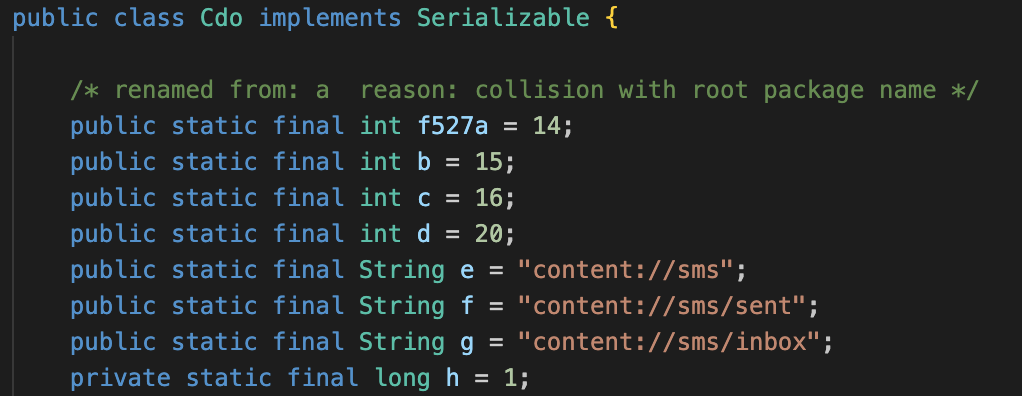
\includegraphics[width=1\textwidth]{./images/screenshot/NaughtyMaid/CDO.png}
    \caption{Cdo}
    \label{fig:CDO}
\end{figure}

\subsubsection{MyTallyUtil and MyCheckUtil}
This two classes are both singleton elements inside the entire project, used to establish a connection to two different remote servers.
After obtaining the singleton object reference through the \texttt{getIns()} method, they both initialize their context with hardcoded values, as it can be seen in Fig. \ref{fig:AppActivityOnCreate}.

The \texttt{pushData} method inside \texttt{MyTallyUtil} starts the execution of an asynchronous task in the background which relays an application identifier and the IMEI code of the phone (Fig. \ref{fig:pushData})

\begin{figure}[h!]
\centering
    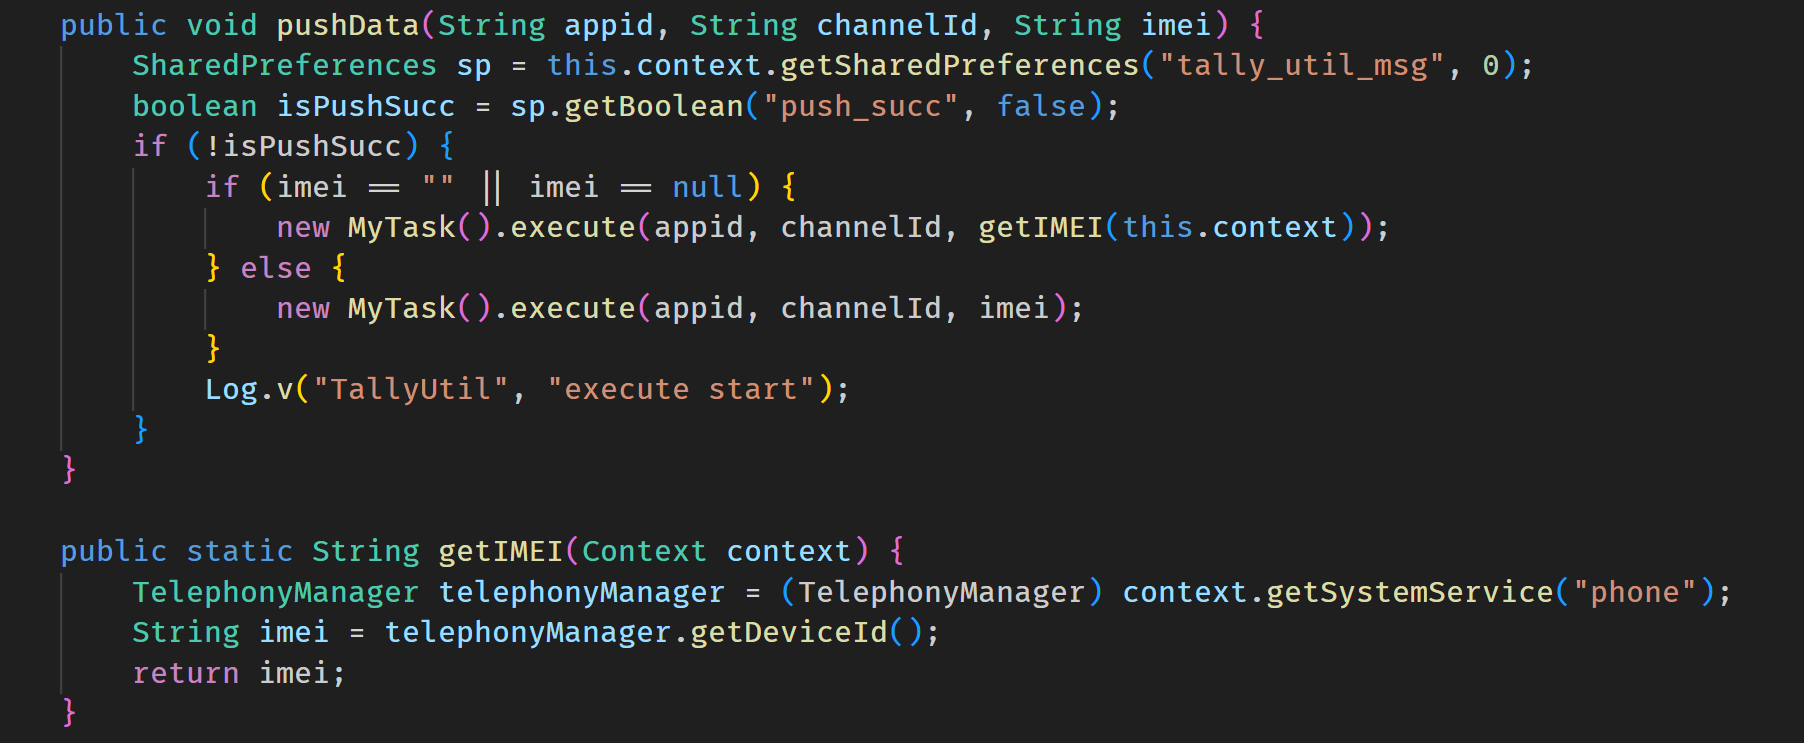
\includegraphics[width=1\textwidth]{./images/screenshot/NaughtyMaid/myTallyUtil-pushData.png}
    \caption{pushData}
    \label{fig:pushData}
\end{figure}

The task performs a simple GET request to the server located at \texttt{www.zhjnn.com:20002}, as shown in Fig \ref{fig:MyTally-MyTask}. When the connection is successful, it remembers it in a shared memory, as to not repeat the connection in future.

The \texttt{receiveData()} method of the \texttt{MyCheckUtil} class, instead, immediately starts the asynchronous task in background, which performs another GET request, this time to the \texttt{web.5ayg.cn:30000} server process (Fig. \ref{fig:mycheckutil-mytask}). The task relays a parameter called \texttt{gameId} and obtains something back, probably a JSON object. This answer is used to set three different flags (obfuscated as a, b, and c) of which, only the third one is used to switch the execution in the main \texttt{AppActivity} as shown in Fig. \ref{fig:callcpp}. The \texttt{callCPP} function is an external one, implemented by the cocos2d library and not directly available by the java decompiler. We assume that it is responsible for loading different versions of the graphical engine part of the application, depending on some characteristics of the device.

\begin{figure}[h!]
\centering
    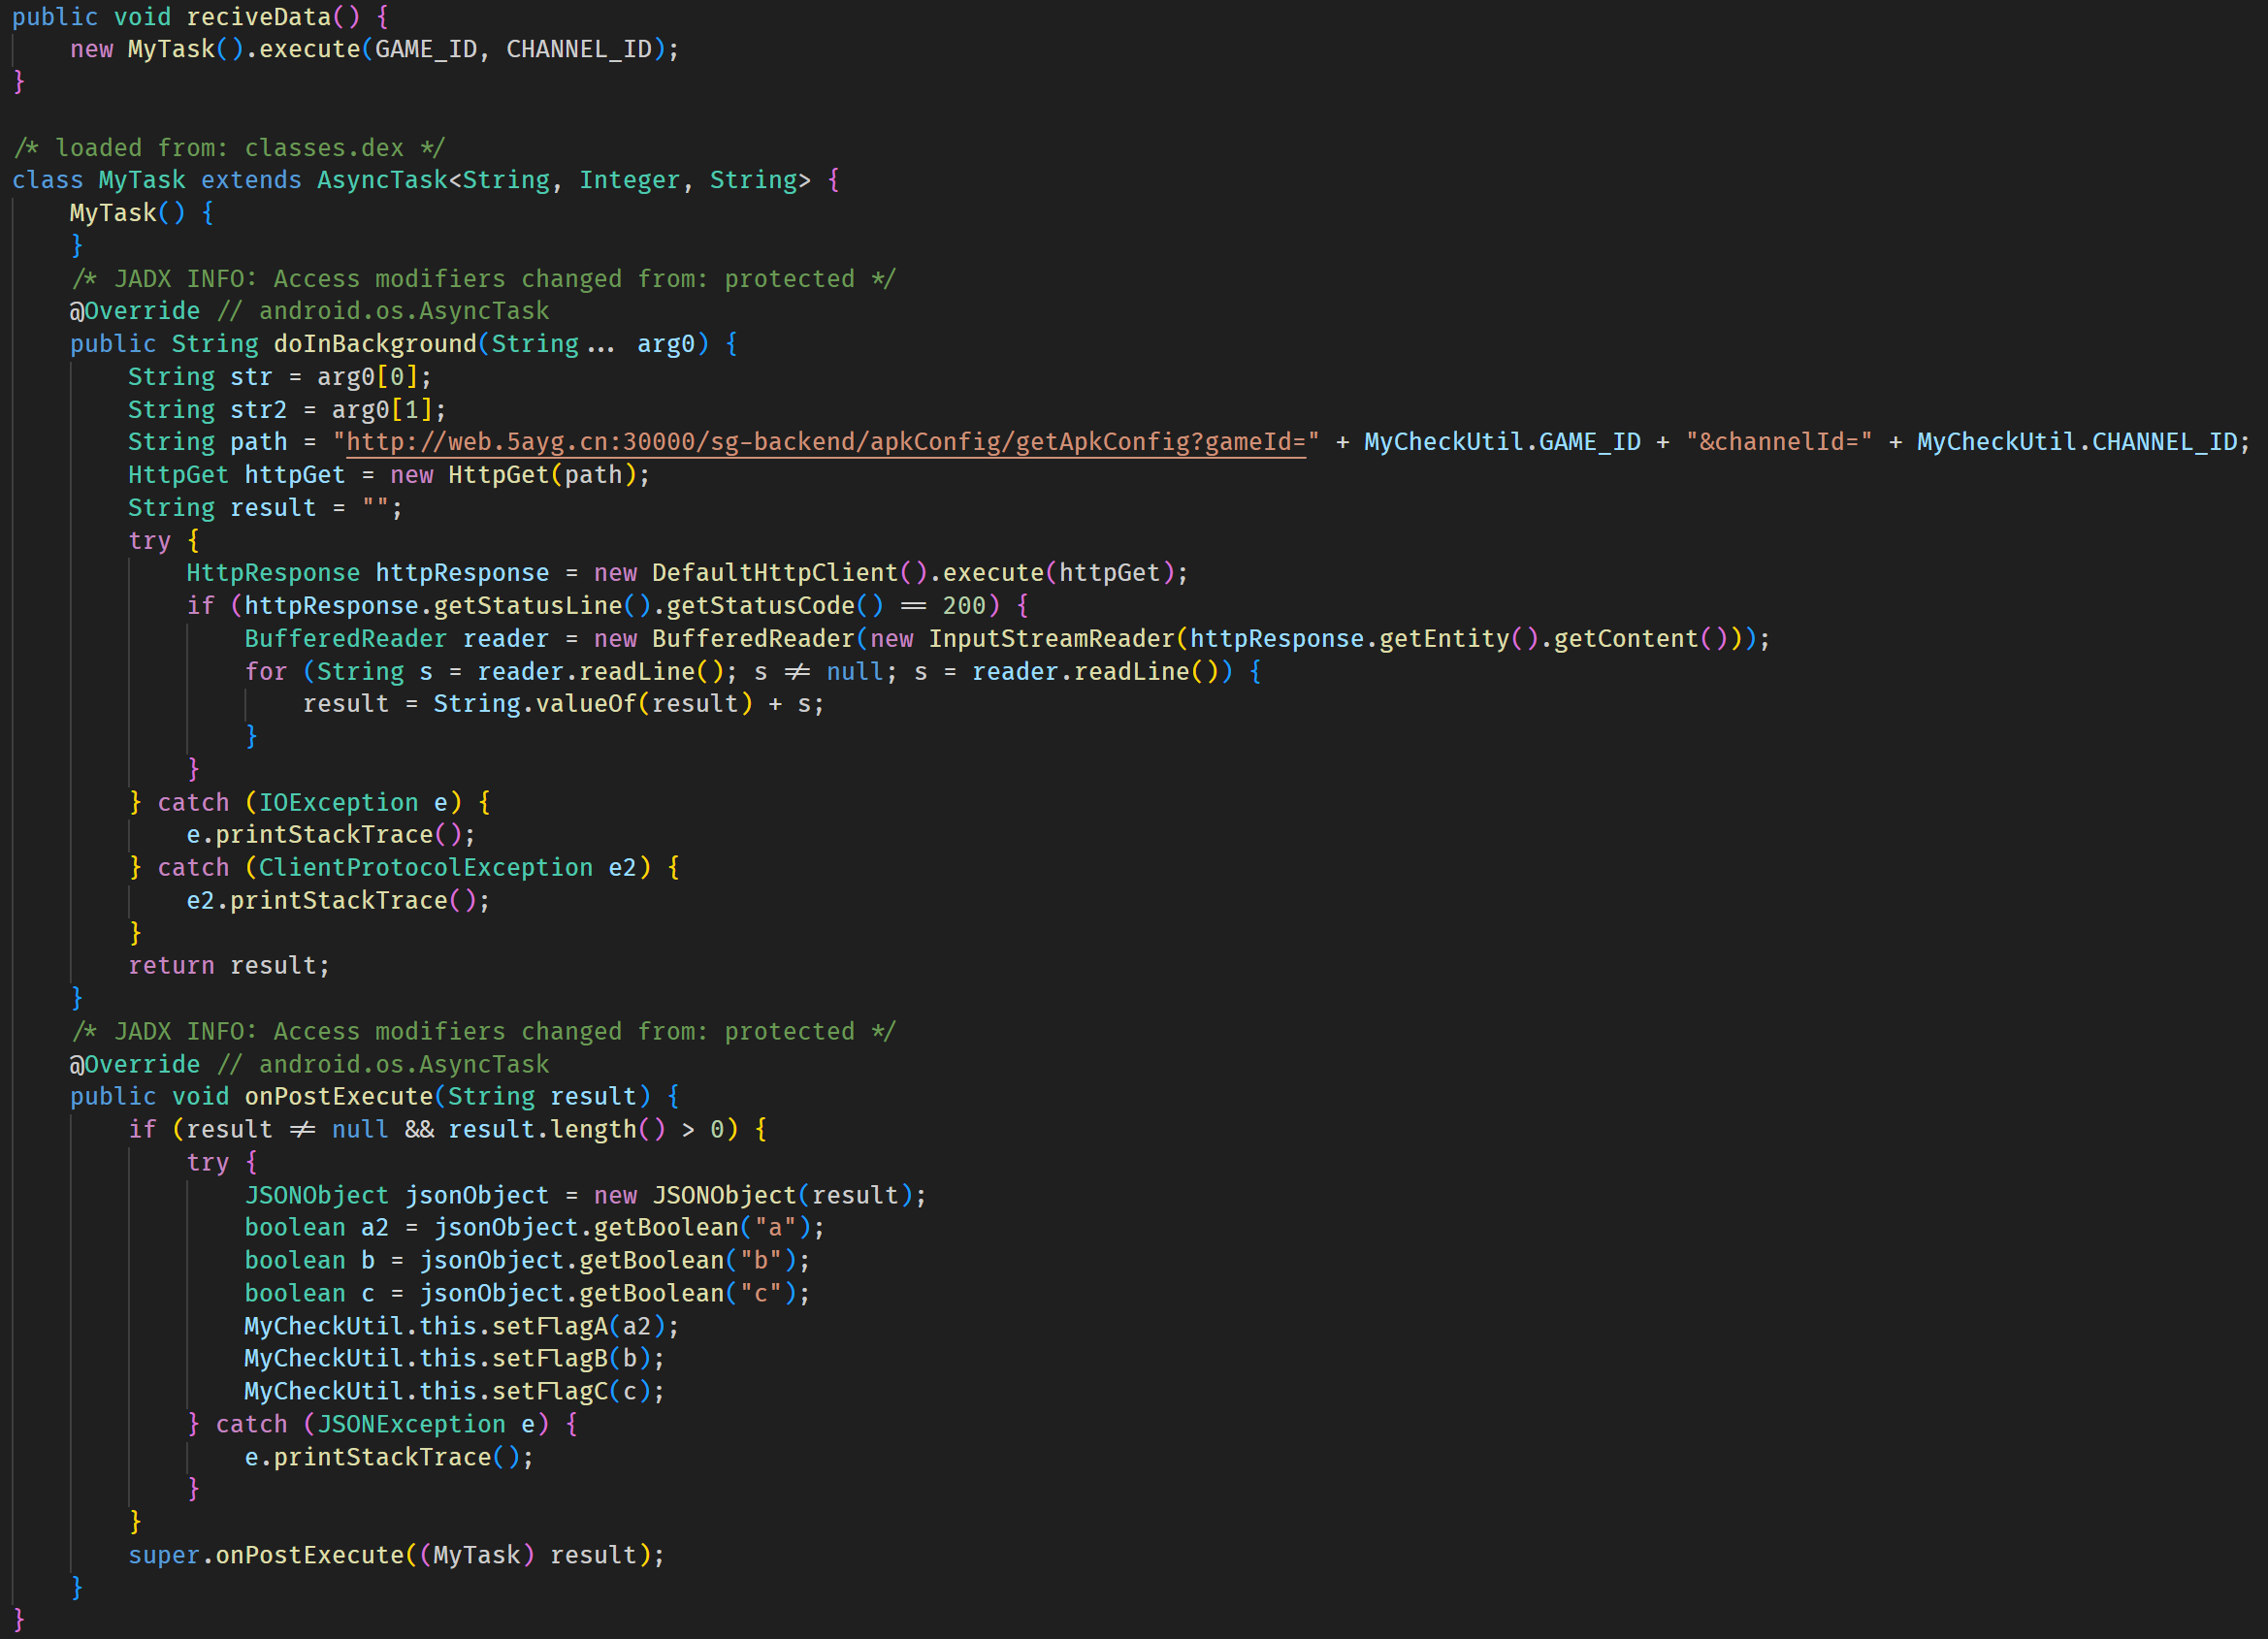
\includegraphics[width=1\textwidth]{./images/screenshot/NaughtyMaid/MyCheckUtil-MyTask.png}
    \caption{MyTask in myCheckUtil}
    \label{fig:mycheckutil-mytask}
\end{figure}

\begin{figure}[h!]
\centering
    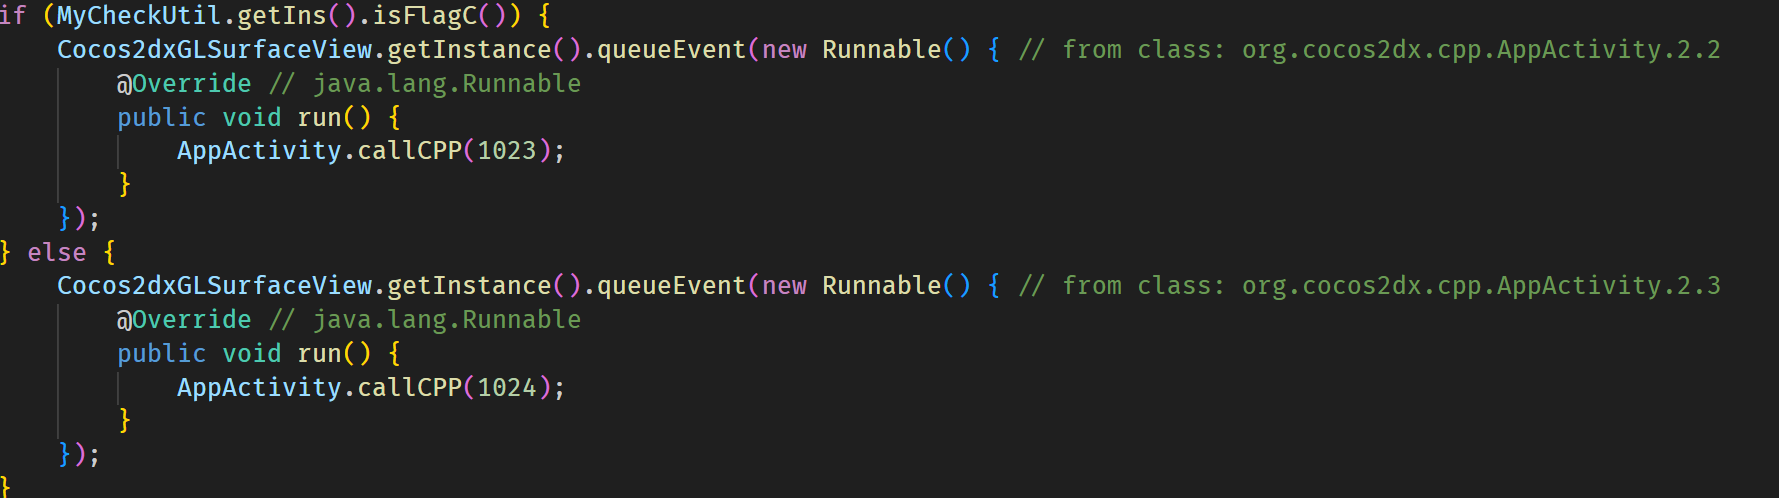
\includegraphics[width=1\textwidth]{./images/screenshot/NaughtyMaid/callCPP-switch.png}
    \caption{different versions of callCPP are called depending on the boolean received by the server}
    \label{fig:callcpp}
\end{figure}

\begin{figure}[h!]
\centering
    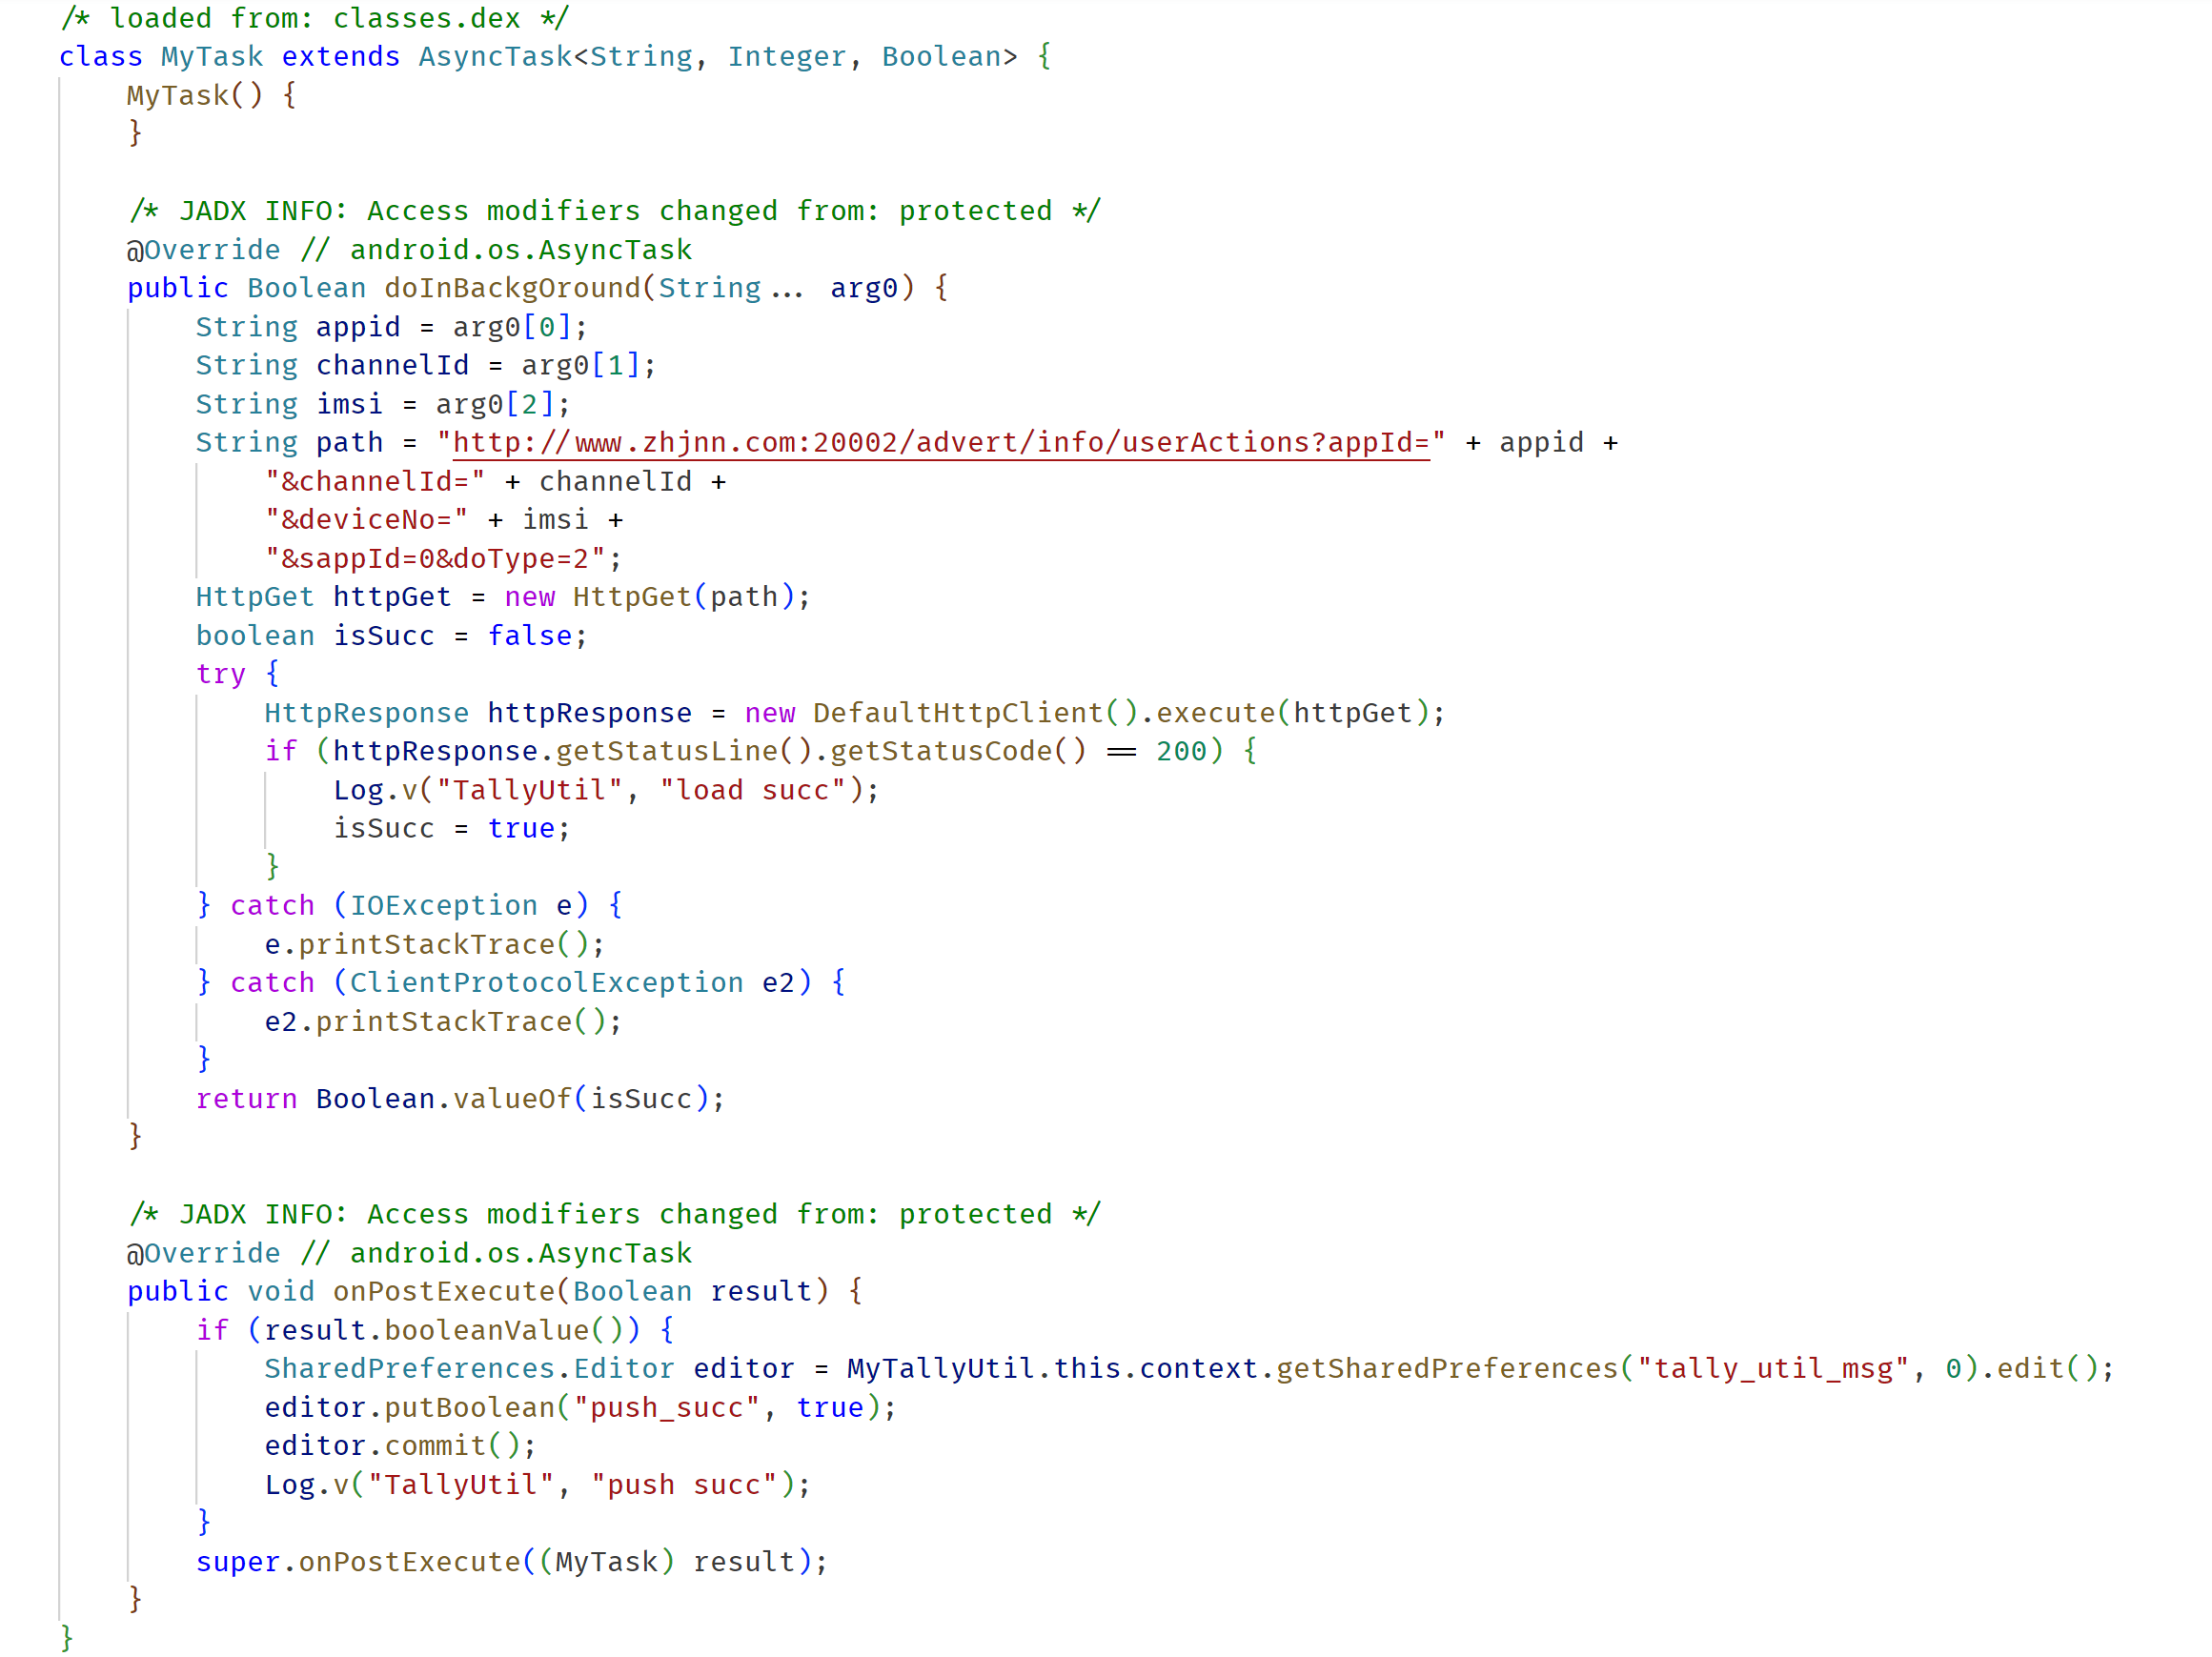
\includegraphics[width=1\textwidth]{./images/screenshot/NaughtyMaid/myTallyUtil-MyTask.png}
    \caption{MyTask in myTallyUtil}
    \label{fig:MyTally-MyTask}
\end{figure}

\subsubsection{Mobclickagent}
Finally, the last operation performed by the \texttt{onCreate} class of \texttt{MyActivity} is to setup a \texttt{MobClickAgent} class. This is part of an SDK service provided by Umeng (\url{https://www.umeng.com/}), a Beijing-based startup, leading provider of mobile app analytics in China. The hard-coded values used to configure this class are therefore a personal token used to identify the application inside the Umeng's web services.